%! Author = adrienkoumgangtegantchouang
%! Date = 07/06/25


% Preamble
\documentclass[a4paper, 12pt]{report}
\usepackage[osf]{libertinus}
\pagestyle{plain}
\usepackage[top=2.5cm,bottom=2.5cm,left=4cm,right=2.5cm, centering]{geometry}
\linespread{1.5}
\usepackage[utf8]{inputenc} % codifica UTF-8
\usepackage{scrlayer-scrpage} % stili pagina per il frontespizio
\pagestyle{scrplain}
\usepackage{mathptmx} % font Times New Roman (simile)
\usepackage{graphicx, wrapfig}
\usepackage{lipsum}

\usepackage{url}
\usepackage{changepage}
\usepackage{multicol}
\usepackage{caption}
\usepackage{subcaption} % For the images' captions
\usepackage[linesnumbered,ruled,vlined]{algorithm2e}
\usepackage{amsmath} % For math symbols
\usepackage{amsthm} % Theorem styles
\usepackage{amssymb} % For special symbols % \mathbb and others
\usepackage{mathrsfs} % An alternative font for categories and sheaves.
\usepackage{cite} % For multiple citations
% \usepackage{caption}
% \usepackage{subcaption} % For the images' captions
\usepackage[section]{placeins} % To not break (sub)-images in two
\usepackage{booktabs}
\usepackage{float} % Always for images
\usepackage{soul} % For the \ul command, to use lists with less vertical spacing
\usepackage{enumerate} % For (i) list style
\usepackage{glossaries}
% \usepackage{minted}

\usepackage{blindtext}
\usepackage{hyperref}

%\usepackage{biblatex} % Imports biblatex package
%\addbibresource{mybibliography.bib} % Import the bibliography file

\usepackage{xcolor} % Optional: for colored code
\renewcommand{\lstlistingname}{Code}% Listing -> Codice\renewcommand{\lstlistingname}{Code}% Listing -> Codice

\usepackage[noend]{algpseudocode}
\algnewcommand\algorithmicforeach{\textbf{for each}}
\algdef{S}[FOR]{ForEach}[1]{\algorithmicforeach\ \#1 \algorithmicdo}

% \usepackage{color}
\usepackage{ragged2e}
\usepackage{algorithmicx}
% \usepackage{algorithm}
% \usepackage{algorithm2e}
\usepackage{program}
% \usepackage{listings-rust}
\usepackage{mathtools}


\usepackage{listings}

\lstdefinestyle{javastyle}{
    language=Java,
    basicstyle=\ttfamily\footnotesize,
    keywordstyle=\color{blue}\bfseries,
    stringstyle=\color{red},
    commentstyle=\color{gray}\itshape,
    numberstyle=\tiny\color{gray},
    backgroundcolor=\color{white},
    numbers=left,
    stepnumber=1,
    numbersep=8pt,
    tabsize=4,
    showspaces=false,
    showstringspaces=false,
    showtabs=false,
    frame=single,
    rulecolor=\color{black},
    captionpos=b,
    breaklines=true,
    breakatwhitespace=true,
    morekeywords={
        String, MapReduce, Mapper, Reducer, Combiner,
        Context, IOException, setup, cleanup,
        Configuration, Job, Text, FileSplit
    },
    literate=
        {<}{{\textless}}1
        {>}{{\textgreater}}1
        {==}{{==}}2
        {!=}{{!=}}2
        {->}{{$\rightarrow$}}2
        {\{}{{\{}}1
        {\}}{{\}}}1,
    escapeinside={(*}{*)},
    xleftmargin=15pt,
    xrightmargin=5pt
}

% In your preamble (with the Java configuration)
\lstdefinestyle{pythonstyle}{
    language=Python,
    basicstyle=\ttfamily\footnotesize,
    keywordstyle=\color{blue}\bfseries,
    stringstyle=\color{red},
    commentstyle=\color{gray}\itshape,
    numberstyle=\tiny\color{gray},
    backgroundcolor=\color{white},
    numbers=left,
    stepnumber=1,
    numbersep=8pt,
    tabsize=4,
    showspaces=false,
    showstringspaces=false,
    showtabs=false,
    frame=single,
    rulecolor=\color{black},
    captionpos=b,
    breaklines=true,
    breakatwhitespace=true,
    morekeywords={
        self, None, True, False, async, await,
        lambda, yield, with, as, from, import
    },
    literate=
        {<}{{\textless}}1
        {>}{{\textgreater}}1
        {\{}{{\{}}1
        {\}}{{\}}}1
        {*}{{\textasteriskcentered}}1
        {/}{{\textbackslash}}1
        {\~}{{\textasciitilde}}1,
    escapeinside={(*}{*)},
    xleftmargin=15pt,
    xrightmargin=5pt,
    alsoletter={@},  % For decorators
    morecomment=[l]{\#},  % Proper single-line comments
    morestring=[b]{"},  % Double quotes
    morestring=[b]{'}   % Single quotes
}


\lstdefinestyle{bashstyle}{
    language=bash,
    basicstyle=\ttfamily\footnotesize,
    keywordstyle=\color{blue}\bfseries,
    stringstyle=\color{red},
    commentstyle=\color{gray}\itshape,
    numberstyle=\tiny\color{gray},
    backgroundcolor=\color{white},
    numbers=left,
    stepnumber=1,
    numbersep=8pt,
    tabsize=4,
    showspaces=false,
    showstringspaces=false,
    showtabs=false,
    frame=single,
    rulecolor=\color{black},
    captionpos=b,
    breaklines=true,
    breakatwhitespace=true,
    morekeywords={
        sudo, apt-get, docker, hadoop, python,
        mkdir, cd, ls, grep, chmod, export
    },
    literate=
        {\$}{{\textcolor{blue}{\$}}}1
        {\#}{{\textcolor{gray}{\#}}}1
        {>}{{\textcolor{red}{\textgreater}}}1
        {|}{{\textcolor{blue}{\textbar}}}1
        {~}{{\textcolor{blue}{\textasciitilde}}}1,
    escapeinside={(*}{*)},
    xleftmargin=15pt,
    xrightmargin=5pt
}


\lstdefinestyle{makefilestyle}{
    language=make,
    basicstyle=\ttfamily\footnotesize,
    keywordstyle=\color{blue}\bfseries,
    stringstyle=\color{red},
    commentstyle=\color{gray}\itshape,
    numberstyle=\tiny\color{gray},
    backgroundcolor=\color{white},
    numbers=left,
    stepnumber=1,
    numbersep=8pt,
    tabsize=4,
    showspaces=false,
    showstringspaces=false,
    showtabs=false,
    frame=single,
    rulecolor=\color{black},
    captionpos=b,
    breaklines=true,
    breakatwhitespace=true,
    morekeywords={
        .PHONY, all, clean, install, test,
        ifeq, ifneq, endif, include, export
    },
    literate=
        {\$}{{\textcolor{blue}{\$}}}1
        {\#}{{\textcolor{gray}{\#}}}1
        {(}{{\textcolor{red}{(}}}1
        {)}{{\textcolor{red}{)}}}1
        {=}{{\textcolor{magenta}{=}}}1,
    sensitive=false, % Make keywords case-insensitive
    alsoletter={-}, % Allow hyphens in target names
    escapeinside={(*}{*)},
    xleftmargin=15pt,
    xrightmargin=5pt,
    moredelim=[s][\color{magenta}]{$(}{)} % Make variables stand out
}



% \usepackage{xcolor}
\definecolor{codegreen}{rgb}{0,0.6,0}
\definecolor{codegray}{rgb}{0.5,0.5,0.5}
\definecolor{codemauve}{rgb}{0.4,0.,0.4}
% \definecolor{codepurple}{rgb}{0.5,0.5,0.5}
% \definecolor{backcolour}{rgb}{0.95,0.95,0.92}

% Define a custom color
\definecolor{backcolour}{rgb}{0.95,0.95,0.92}
\definecolor{codegreen}{rgb}{0,0.6,0}
\definecolor{codekeywork3}{rgb}{0.82,0.56,0.43}
% Define a custom style


\definecolor{jsonbackground}{RGB}{245,245,244}
\definecolor{jsonstring}{RGB}{173,0,0}
\definecolor{jsonkey}{RGB}{0,0,180}
\definecolor{jsoncomment}{RGB}{85,85,85}
\definecolor{jsonnumber}{RGB}{128,64,0}

\lstdefinelanguage{json}{
    basicstyle=\ttfamily\footnotesize,
    numbers=left,
    numberstyle=\tiny\color{gray},
    stepnumber=1,
    numbersep=8pt,
    showstringspaces=false,
    breaklines=true,
    frame=single,
    backgroundcolor=\color{jsonbackground},
    string=[s]{"}{"},
    comment=[l]{//},
    morecomment=[s]{/*}{*/},
    literate=
        *{:}{{{\color{black}:}}}{1}
        {,}{{{\color{black},}}}{1}
        {\{}{{{\color{black}{\{}}}}{1}
        {\}}{{{\color{black}{\}}}}}{1}
        {[}{{{\color{black}[}}}{1}
        {]}{{{\color{black}]}}}{1}
    keywordstyle=\color{jsonkey}\bfseries,
    stringstyle=\color{jsonstring},
    commentstyle=\color{jsoncomment}\itshape
}


\newtheorem{mydef}{Definition}
\newtheorem{mytheo}{Theorem}
\newtheorem{mylem}{Lemma}
\newtheorem{mypro}{Property}
\newtheorem{myex}{Example}
\newtheorem{mycor}{Corollary}
\newtheorem{myproof}{Proof idea}
\newtheorem{mypc}{Pseudocode}


\usepackage{tabularx}


\begin{document}
    %! Author = adrienkoumgangtegantchouang
%! Date = 07/06/25

\begin{titlepage} %crea l'enviroment
\begin{figure}[t] %inserisce le figure
    \centering
\includegraphics[width=0.70\textwidth]{marchio_unipi_pant541}\label{fig:figure-first-page}
\end{figure}

\begin{figure}[t] %inserisce le figure
    \centering
\includegraphics[width=0.60\textwidth]{DII Logo}\label{fig:figure-first-page-2}
\end{figure}

\vspace{5mm}

\begin{Large}
 \begin{center}
	\textbf{Master's Degree in Artificial Intelligence and Data Engineering\\}
	\vspace{7mm}
    {\Large{Design and develop of an Application interacting with NoSQL Databases:}}\\
	\vspace{2mm}
	{\LARGE{\textbf{Smart News Aggregator}}}
\end{center}
\end{Large}

\vspace{10mm}

%minipage divide la pagina in due sezioni settabili
\begin{minipage}[t]{0.47\textwidth}
	{\large{\textbf{Instructors:\\ Prof. Pietro Ducange \\ Prof. Alessio Schiavo}}}
\end{minipage}
\hfill
\begin{minipage}[t]{0.47\textwidth}\raggedleft
	{\large{\textbf{Student: \\ Adrien Koumgang Tegantchouang}}}
\end{minipage}

\vspace{20mm}

\centering{\large{\textbf Academic Year 2024/2025}}

\end{titlepage}


    \tableofcontents


    \thispagestyle{empty}

    \clearpage
    \setcounter{page}{1}


% Introduction
    %! Author = adrienkoumgangtegantchouang
%! Date = 08/06/25


\chapter{Introduction}\label{ch:introduction}


\section{Overview}\label{sec:overview}

In the digital age, the volume of news articles produced every day is staggering.
Readers are increasingly overwhelmed by the amount of available content and often struggle to find reliable and relevant information that matches their personal interests.
To address this challenge, we propose the development of a \textbf{Smart News Aggregator & Reader Personalization Platform}.

This platform collects news articles from multiple external APIs, stores and processes them using NoSQL databases (MongoDB and Redis), and delivers a personalized reading experience to users.
It incorporates intelligent recommendation features, secure user authentication via JWT tokens, and real-time analytics to improve user engagement.


\section{Objectives}\label{sec:objectives}

The primary objective of this project is to \textbf{design and implement a distributed news aggregation application} of intelligently retrieving,
storing, analyzing, and serving large-scale multi-structured data using multiple NoSQL database technologies.

In line with the course requirements for \textbf{Large Scale and Multi-Structured Databases}, the specific goals of this project include:

\begin{itemize}
    \item \textbf{Data Acquisition \& Preprocessing}: Retrieve a real-world, high-volume dataset ($\leg$ 50MB) from multiple external news APIs (e.g., MediaStack, newsData, The Guardian, NYTimes), ensuring \textbf{variety} and \textbf{velocity}.
    \item \textbf{Distributed NoSQL Architecture}: Use \textbf{MongoDB} as the primary \textbf{Document Database}, with carefully designed collections, indexes, and aggregation pipelines.
    Integrate a \textbf{Key-Value store} (\textbf{Redis}) to optimize caching and access to hot data.
    \item \textbf{System Design and Modeling}: Define functional and non-functional requirements.
    Design UML class diagrams and user interface mockups.
    Model the data schema for each NoSQL DB in use.
    \item \textbf{RESTful API Backend}: Build a scalable backend using Flask and Flask-RESTX.
    Expose secure endpoints with JWT-based authentication.
    Provide API documentation via Swagger and test interfaces.
    \item \textbf{Advanced Analytics}: Implement at least three real aggregation pipelines in MongoDB for summarizing and analyzing article content and user activity.
    Provide user-personalized views and filtering using advanced queries.
    \item \textbf{Monitoring, Testing, and Depployment}: Deploy on both and UNIPI virtual clusters.
    Include performance tests, system logging, and analysis of read/write throughput under different consistency models.
    Offer a complete presentation and demonstration, including API functionality and analytics insights.
\end{itemize}

By achieving these goals, the project demonstrates my ability to handle real-world large-scale data applications,
integrating theoretical design with practical deployment, and ensuring cross-database consistency and performance.


\section{Structure of the presentation}\label{sec:structure-of-the-presentation}

The documentation is structured as follows:

\begin{itemize}
    \item \textbf{Chapter 1 - Introduction}: Presents the context, objectives, and structure of the project, outlining the motivations and academic scope.
    \item \textbf{Chapter 2 - Requirements Analysis}: Identifies the functional and non-functional requirements of the application, defines the system actors, and outlines key use cases.
    \item \textbf{Chapter 3 - System Design}: Includes the architectural overview, UML class diagrams, and mockup wireframes of the application’s user interface.
    \item \textbf{Chapter 4 - NoSQL Database Modeling}: Describes the design choices for MongoDB (Document DB) and Redis (Key-Value DB), along with schema definitions, key structures, and CAP theorem considerations.
    \item \textbf{Chapter 5 - Data Ingestion and Integration}: Explains how external APIs are connected, data is fetched and transformed, and stored into the databases.
    Also includes logging and handling of errors and API rate limits.
    \item \textbf{Chapter 6 - Backend Implementation}: Details the development of RESTful API endpoints using Flask and Flask-RESTX, JWT authentication, Swagger documentation, and the modular blueprint structure.
    \item \textbf{Chapter 7 - Advanced Aggregations and Analytics}: Presents non-trivial aggregation pipelines in MongoDB, user-specific personalization features, and analytics insights extracted from the dataset.
    \item \textbf{Chapter 8 - Deployment and Testing}: Discusses deployment on local and virtualized environments, performance testing scenarios, and consistency benchmarking across NoSQL systems.
    \item \textbf{Chapter 9 - Conclusion}: Summarizes achievements, reflects on encountered challenges, and suggests possible extensions to improve scalability, interactivity, and intelligence.
\end{itemize}



% Requirements Analysis
    %! Author = adrienkoumgangtegantchouang
%! Date = 08/06/25


\chapter{Requirements Analysis}\label{ch:requiremnts-analysis}


\section{Problem Statement}\label{sec:problem-statement}

With the exponential growth of online content, users are overwhelmed by the volume of news available across platforms.
This leads to difficulty in identifying relevant and trustworthy information.
The proposed system aims to aggregate articles from various news APIs and personalize the reading experience based on user behavior and preferences, while maintaining scalability and high performance.


\section{Stackeholders and Actors}\label{sec:stackeholders-actors}

The successful deployment and functioning of the Smart News Aggregator \& Reader Personalization Platform depends on multiple stakeholders and actors who interact directly or indirectly with the system.
This section outlines their roles and responsibilities.

\subsection{Stackeholders}\label{subsec:stackeholders}

\begin{itemize}
    \item \textbf{End Users}: Consume and interact with news content; expect personalized and relevant information.
    \item \textbf{Platform Administrator}: Oversees user activity, ensures data integrity, and manages access or moderation tasks.
    \item \textbf{Project Developers}: Build and maintain the system backend, frontend, and data processing pipelines.
    \item \textbf{External API Providers}: Supply news content (e.g., NYTimes, Guardian, NewsData, CurrentsAPI, MediaStack).
    \item \textbf{Academic Supervisors}: Oversee the project's architecture, correctness, and evaluate its educational objectives.
\end{itemize}

\subsection{Actors}\label{subsec:actors}

\begin{itemize}
    \item \textbf{Visitor (Anonymous user)}: Accesses the welcome page and Can register to become a user.
    \item \textbf{Registered User}: Logs into the platform, Personalizes preferences, Views news feed and Interacts with articles (like/comment).
    \item \textbf{Administrator}: Manages users and platform configurations and Monitors logs and analytics.
    \item \textbf{News Aggregator Service}: Fetches articles from external APIs and Normalizes and stores them into MongoDB.
    \item \textbf{External News APIs}: Provide raw article data in JSON format for ingestion by the system.
\end{itemize}

Each actor has specific actions and permissions that are further detailed in the Use Case and UML Diagrams.


\section{Functional Requirements}\label{sec:functional-requirments}

The Smart News Aggregator \& Reader Personalization Platform offers a suite of functionalities that serve both user-facing and administrative purposes.
The following functional requirements have been identified:

\subsection{User Account Management}\label{subsec:user-account-management}

\begin{itemize}
    \item \textbf{Registration}: Users must be able to register with valid email and password.
    \item \textbf{Login/Logout}: Authenticated access via JWT-based login; logout clears session on frontend.
    \item \textbf{Profile Management}: Users can update personal data (e.g., name, preferences).
    \item \textbf{Password Handling}: Secure password storage and update with history tracking.
\end{itemize}

\subsection{News Aggregation \& Display}\label{subsec:news-aggregation-diplay}

\begin{itemize}
    \item \textbf{Fetch Articles from External APIs}: The system retrieves and normalizes article data from third-party providers such as NYTimes, NewsData, CurrentsAPI, etc.
    \item \textbf{Categorized News Display}: Articles are displayed by category (e.g., politics, tech, sports).
    \item \textbf{Search \& Filter}: Users can search articles using keywords and filter by category, source, or date.
    \item \textbf{Pagination}: Article lists are paginated to handle large datasets.
\end{itemize}

\subsection{Personalization \& Recommendation}\label{subsec:personalization-recommendation}

\begin{itemize}
    \item \textbf{Save Preferences}: Users can set preferred categories, sources, or languages.
    \item \textbf{Personalized Feed}: Articles are filtered and ranked based on user preferences.
    \item \textbf{Like \& Save Articles}: Users can like or save articles for future reading.
    \item \textbf{Commenting System}: Users can add comments and replies to articles.
\end{itemize}

\subsection{Admin \& Analytics}\label{subsec:admin-analytics}

\begin{itemize}
    \item \textbf{Dashboard Access}: Admin can view usage statistics and system logs.
    \item \textbf{User Management}: Admin can deactivate or delete user accounts.
    \item \textbf{API Health Monitoring}: Admin is notified of errors when external APIs fail.
    \item \textbf{Article Quality Control}: Admin can remove duplicated or malformed articles.
\end{itemize}

\subsection{System \& Logging}\label{subsec:system-logging}

\begin{itemize}
    % \item \textbf{API Logging}: All requests to critical endpoints are logged (including metadata like headers and response time).
    \item \textbf{Authentication Event Logs}: Login/Logout attempts are store for audit.
    \item \textbf{Error Tracking}: Failed requests or errors are stored in MongoDB.
\end{itemize}


\section{Non-Functional Requirements}\label{sec:non-functional-requirements}

This section outlines the quality attributes and constraints the Smart News Aggregator \& Reader Personalization Platform must meet to ensure reliability, security, and scalability.

\subsection{Performance}\label{subsec:performance}

The system must handle a high number of concurrent users with minimal latency.
Article feed pages must load within 1 second under normal network conditions.
External API data must be cached using Redis to reduce response time and load.


\subsection{Scalability}\label{subsec:scalability}

The backend architecture must support horizontal scaling to accommodate growing numbers of users and API integrations.
MongoDB and Redis must be configured to handle large-scale document and key-value datasets efficiently.

\subsection{Availability}\label{subsec:availability}

The application must ensure high availability (99.9\%) during user access hours.
In the case of third-party API failure, the system should provide fallback responses or cached data when available.

\subsection{Security}\label{subsec:security}

User authentication must use JWT with asymmetric encryption (RS256).
Passwords must be securely hashed (using bcrypt) and stored with history to prevent reuse.
All endpoints must enforce token validation for sensitive operations.
Cross-Origin Resource Sharing (CORS) must be properly configured to restrict access to allowed domains.

\subsection{Maintainability}\label{subsec:maintainability}

The system must be modular, separating concerns by feature (auth, articles, users).
Logging and exception handling must be centralized to simplify debugging and maintenance.
Code must be written following best practices and TypeScript (frontend) and Python (backend) style guides.

\subsection{Usability}\label{subsec:usability}

The frontend must offer an intuitive user interface with minimal learning curve.
Responsive design must ensure accessibility on desktops, tablets, and mobile devices.

\subsection{Portability}\label{subsec:portability}

The application must run on Unix-based systems and be container-ready (Docker-compatible).
APIs must be documented using Swagger/OpenAPI to allow easy integration by external systems.


\section{Use Case Diagrams}\label{sec:use-case-diagrams}

These diagrams were created using PlantUML\@.

%\begin{figure}[!h]
%    \centering
%    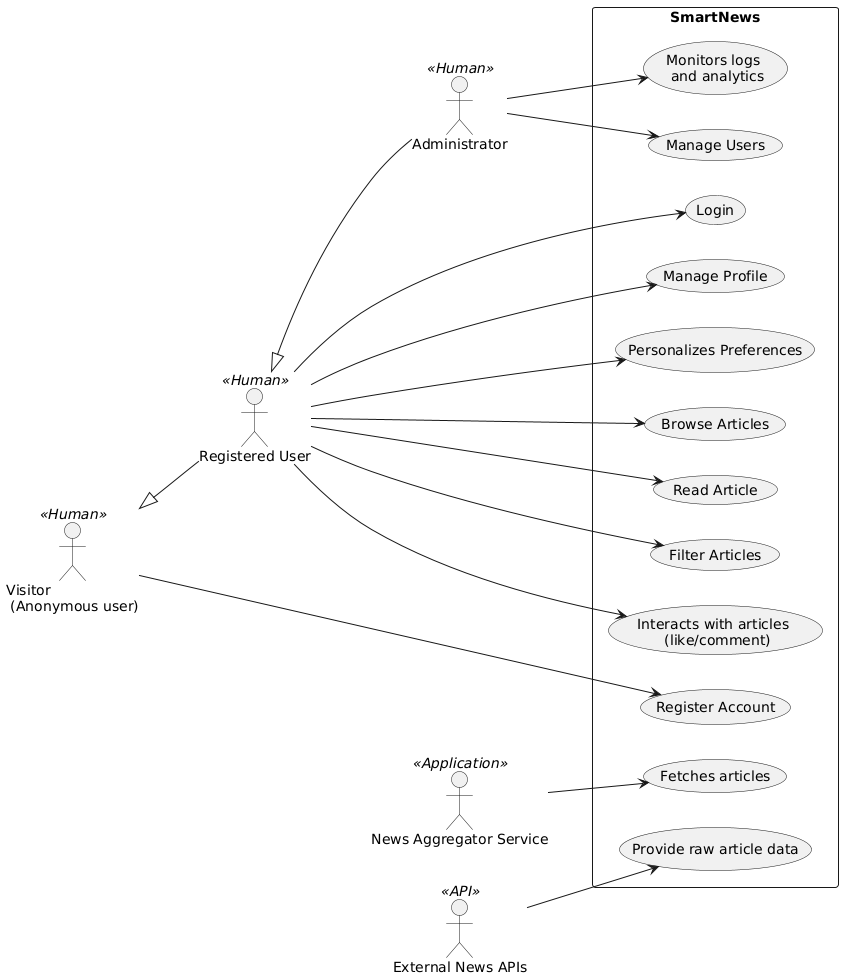
\includegraphics[width=1.1\textwidth]{chapters/chapter_02/diagram-sn-uml-2}
%    \caption{Use Case Diagram}
%    \label{fig:use-case-diagram}
%\end{figure}


\begin{figure}[!h]
    \centering
    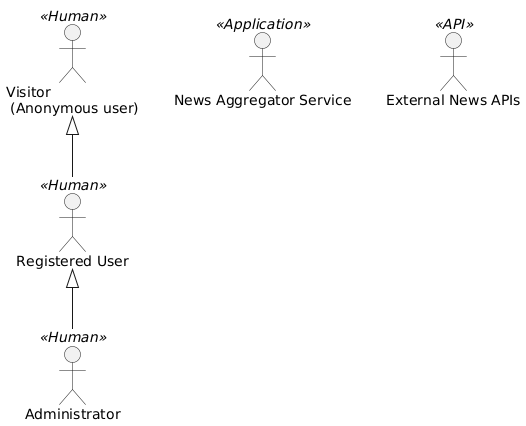
\includegraphics[width=0.5\textwidth]{chapters/chapter_02/use-case-smart-news-actors}
    \caption{Use Case Diagram : Actors}
    \label{fig:use-case-diagram-actors}
\end{figure}


\begin{figure}[!h]
    \centering
    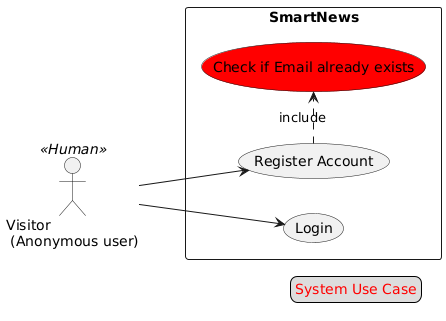
\includegraphics[width=0.5\textwidth]{chapters/chapter_02/use-case-smart-news-anonymous-user}
    \caption{Use Case Diagram: Anonymous User}
    \label{fig:use-case-diagram-anonymous-user}
\end{figure}


\begin{figure}[!h]
    \centering
    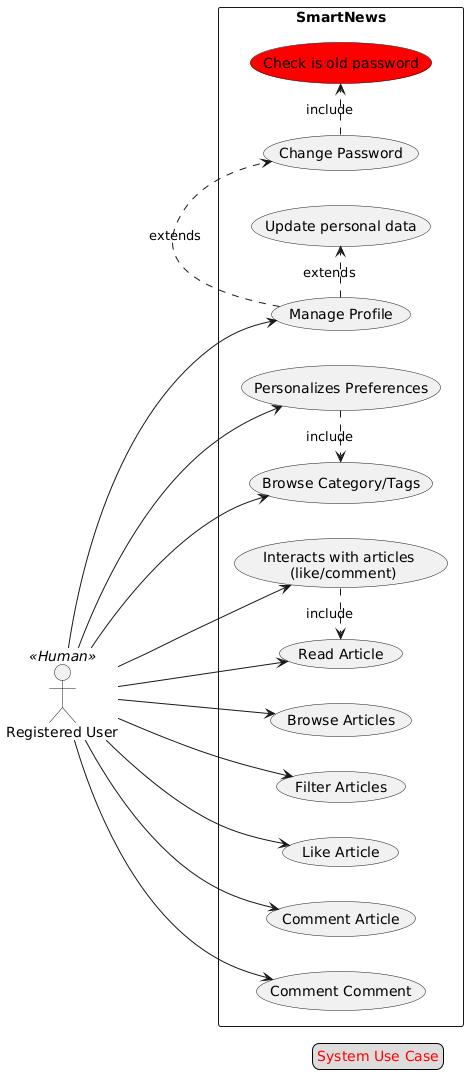
\includegraphics[width=0.5\textwidth]{chapters/chapter_02/use-case-smart-news-registered-user}
    \caption{Use Case Diagram: Registered User}
    \label{fig:use-case-diagram-registered-user}
\end{figure}


\begin{figure}[!h]
    \centering
    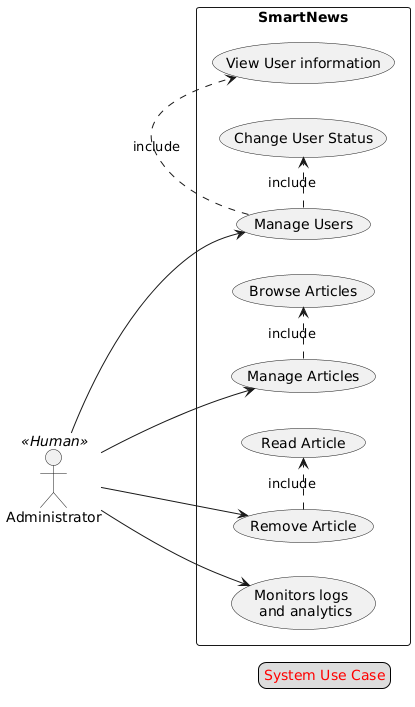
\includegraphics[width=0.5\textwidth]{chapters/chapter_02/use-case-smart-news-administrator}
    \caption{Use Case Diagram: Administrator}
    \label{fig:use-case-diagram-administrator}
\end{figure}


\begin{figure}[!h]
    \centering
    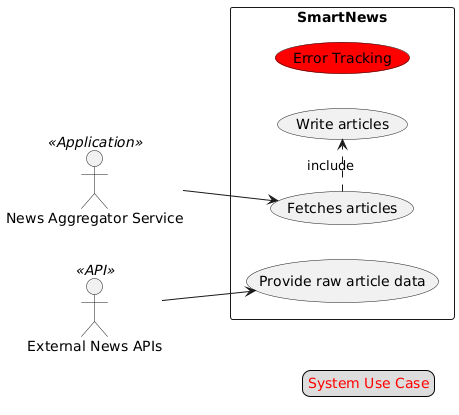
\includegraphics[width=0.5\textwidth]{chapters/chapter_02/use-case-smart-news-system}
    \caption{Use Case Diagram: Systen}
    \label{fig:use-case-diagram-system}
\end{figure}





% System Design
    %! Author = adrienkoumgangtegantchouang
%! Date = 08/06/25


\chapter{System Design}\label{ch:system-design}


This chapter presents the architectural and structural design of the Smart News Aggregator \& Reader Personalization Platform.
It includes a high-level system architecture, database modeling strategy, UML class diagrams, and mockups of key user interfaces.


\section{Architecture Overview}\label{sec:architecture-overview}

The platform is built using a \textbf{modular and layered architecture} to separate concerns and ensure maintainability, performance, and scalability.
It integrates multiple technologies:

\subsection{Key Components}\label{subsec:key-components}

\begin{itemize}
    \item \textbf{Frontend (React\cite{react, vite} + TypeScript)}: Handles UI, user interaction, API communication and Token-based authentication.
    \item \textbf{Backend (Flask + Flask-RESTX)}: RESTful API with Blueprint organization, JWT authentication with RS256 and Logging and error handling.
    \item \textbf{Document Database (MongoDB)}: Stores user profiles, articles, comments, and logs.
    Supports complex queries and aggregation pipelines.
    \item \textbf{Key-Value Store (Redis)}: Caches trending articles and recent queries.
    Session tracking.
    \item \textbf{External APIs}: Article data sources such as CurrentsAPI, NewsData, NYTimes, Guardian.
\end{itemize}


\section{System Architecture Diagram}\label{sec:system-architecture-diagram}

The architecture is divided into four layers:
\begin{itemize}
    \item \textbf{Client Layer}: Browser-based React frontend
    \item \textbf{Application Layer}: Flask server handling HTTP requests, routing, and validation
    \item \textbf{Data Layer}: MongoDB for structured content, Redis for quick key access
    \item \textbf{External Sources}: Third-party APIs for news ingestion
\end{itemize}


\begin{figure}[!h]
    \centering
    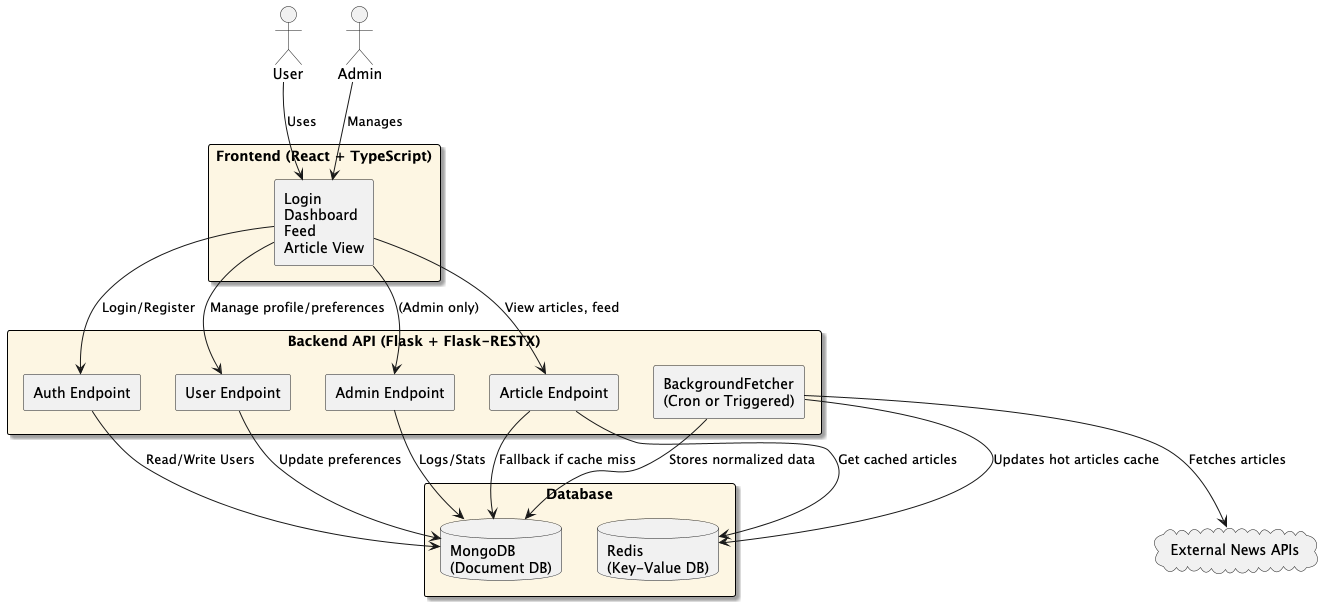
\includegraphics[width=1.1\textwidth]{chapters/chapter_03/system-architecture-smart-news-aggregator}
    \caption{System Architecture}
    \label{fig:system-architecture-diagram}
\end{figure}

\subsection{Client Layer (Frontend)}\label{subsec:client-layer-frontend}

At the forefront is the \textbf{Client Layer}, which consists of a web-based frontend developed using React and TypeScript.
This layer handles the user interface, manages routing, and communicates with the backend API through Axios.
JWT tokens are stored in the browser’s localStorage for session management.
Users interact with interfaces such as login, registration, the personalized news feed, article detail views, and, for administrators, a dedicated dashboard.

\subsection{Application Layer (Flask Backend)}\label{subsec:application-layer-flask-backend}

The \textbf{Application Layer} is built on Flask with Flask-RESTX to expose RESTful endpoints in a modular architecture.
This layer is responsible for authenticating users using asymmetric JWT (RS256), routing client requests to appropriate service handlers, and managing background tasks like scheduled fetching of articles.
It includes modules like auth\_endpoint, user\_endpoint, article\_endpoint, and admin\_endpoint, as well as libraries for handling authentication keys and logging system events into MongoDB\@.

\subsection{Data Layer}\label{subsec:data-layer}

The \textbf{Data Layer} integrates two complementary NoSQL technologies.
MongoDB, as a document-oriented database, is used to store structured collections such as users, articles, comments, preferences, and system logs.
It supports advanced aggregation pipelines and enables efficient historical analysis.
Redis, on the other hand, serves as a key-value store optimized for performance.
It caches the latest articles, manages trending topics, and supports rate limiting.
Redis ensures low-latency data access and reduces the load on MongoDB for repetitive queries.

\subsection{External APIs Layer}\label{subsec:external-apis-layer}

At the periphery, the \textbf{External APIs Layer} includes third-party news services like MediaStack, CurrentsAPI, NewsData, the New York Times API, and the Guardian API\@.
A background fetcher service, either scheduled or triggered, connects to these APIs, retrieves articles, normalizes the data, and saves the cleaned results into MongoDB\@.
This ensures that the content database is continuously updated with fresh news.

\vspace{2cm}

The data flow follows a secure and performance-driven path.
When a user logs in, they are authenticated via JWT, and the token is returned in the Authorization header.
The frontend then retrieves the latest articles by calling the /article/latest endpoint.
If the content is cached in Redis, it is served directly; otherwise, Flask queries MongoDB. Meanwhile, the background fetcher periodically updates the article repository.
Personalized recommendations are generated by combining user preferences with MongoDB aggregations and Redis-cached data.
Administrators can monitor platform activity and user engagement via metrics obtained through aggregation queries stored in MongoDB\@.

\section{UML Class Diagram}\label{sec:uml-class-diagram}

\begin{figure}[!h]
    \centering
    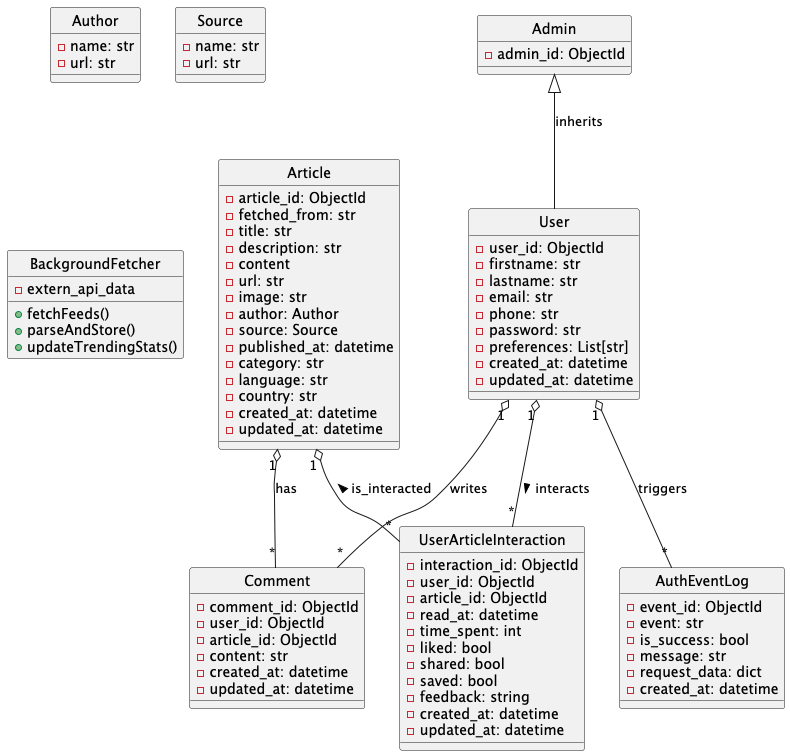
\includegraphics[width=1\textwidth]{chapters/chapter_03/uml-class-diagram}
    \caption{Use Case Diagram: Systen}
    \label{fig:uml-class-diagram}
\end{figure}




\section{UI Wireframes and Mockups}\label{sec:ui-wireframes-and-mockups}

\subsection{Authentication Screens}\label{subsec:authentication-screens}

For registered new user and login:

\begin{figure}[!h]
    \centering
    \begin{minipage}{0.48\linewidth}
        \centering
        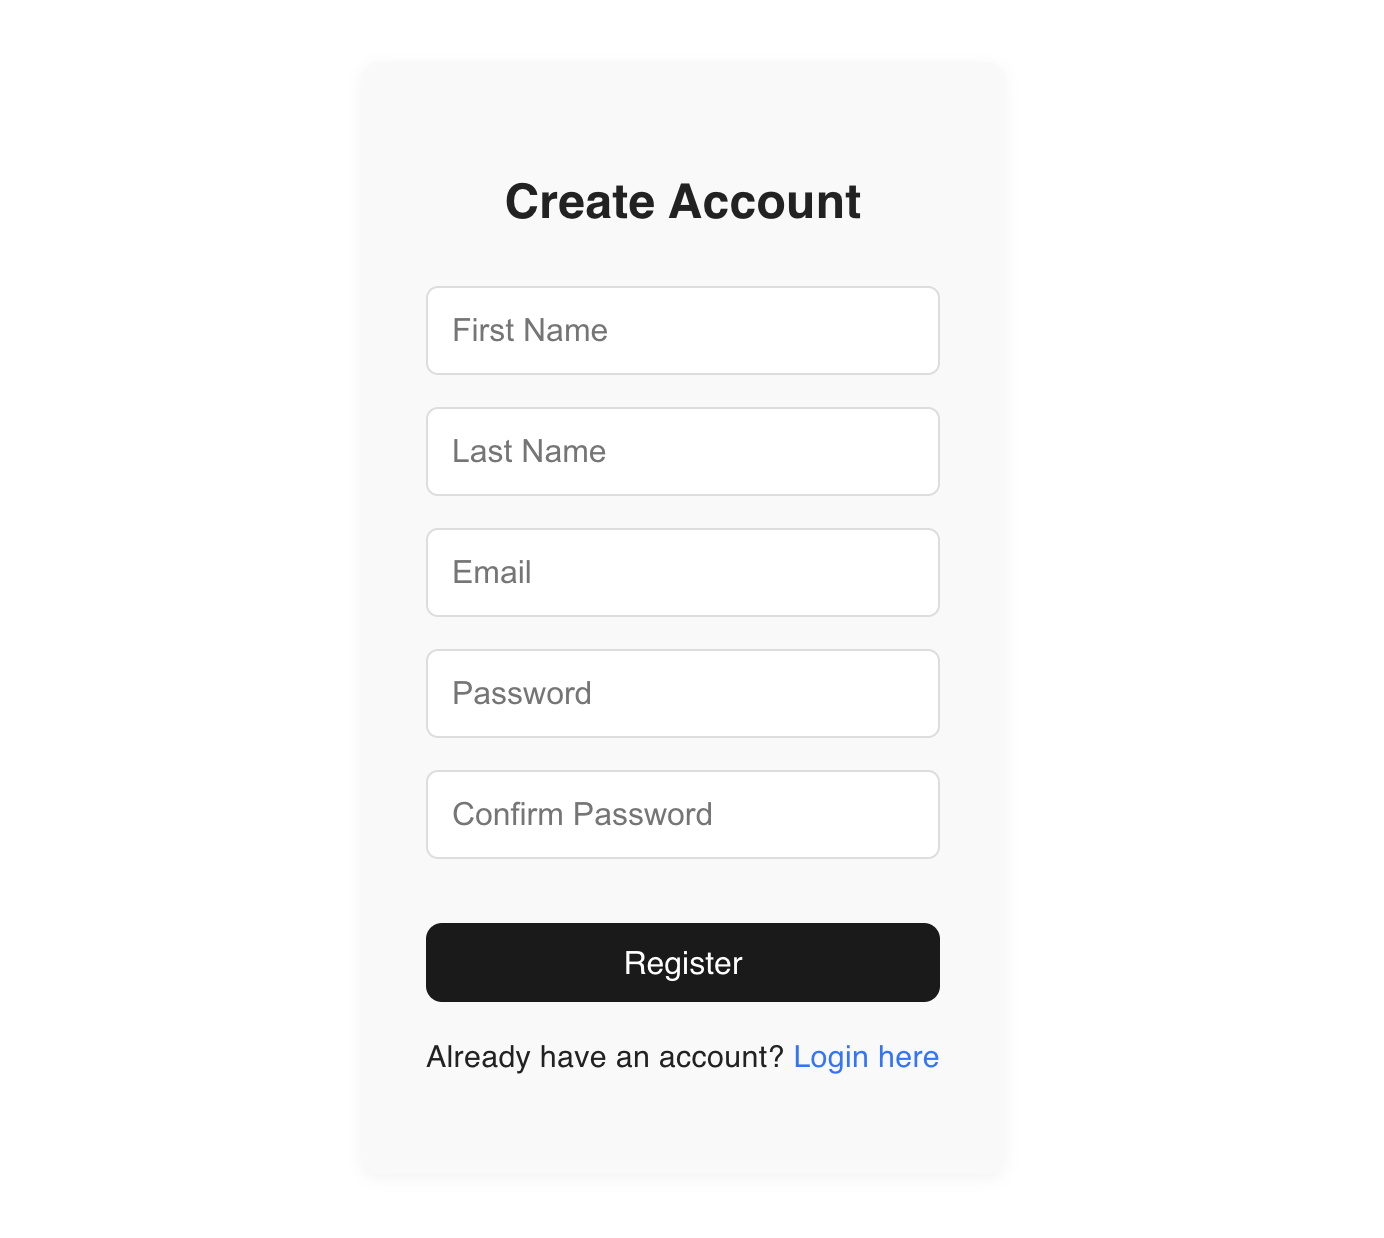
\includegraphics[width=1\textwidth]{chapters/chapter_03/page/auth/register-page}
        \caption{Authentication screens: registration page}
        \label{fig:registration-wireframes}
    \end{minipage}
    \hfil
    \begin{minipage}{0.48\linewidth}
        \centering
        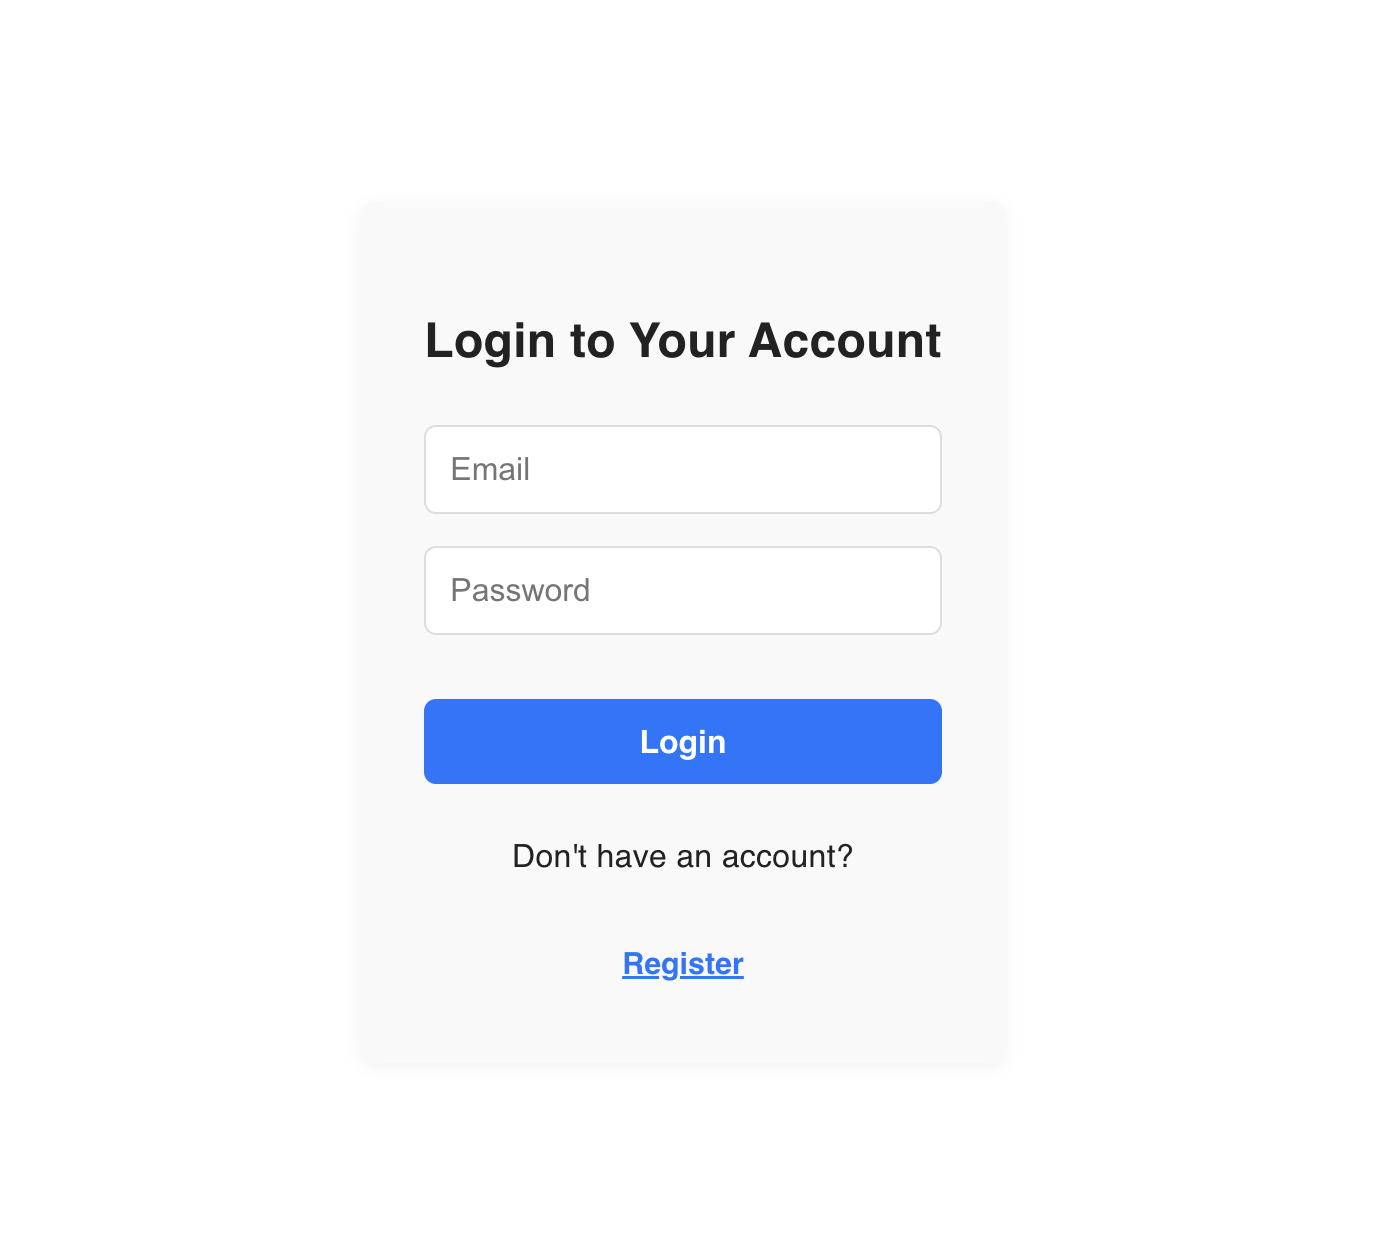
\includegraphics[width=1\textwidth]{chapters/chapter_03/page/auth/login-page}
        \caption{Authentication screens: login page}
        \label{fig:login-wireframes}
    \end{minipage}
\end{figure}


\subsection{User Screens}\label{subsec:user-screens}

For see user all user information.
It's not possible for user with role "user" to modify status and role.

\begin{figure}[!h]
    \centering
    \begin{minipage}{0.48\linewidth}
        \centering
        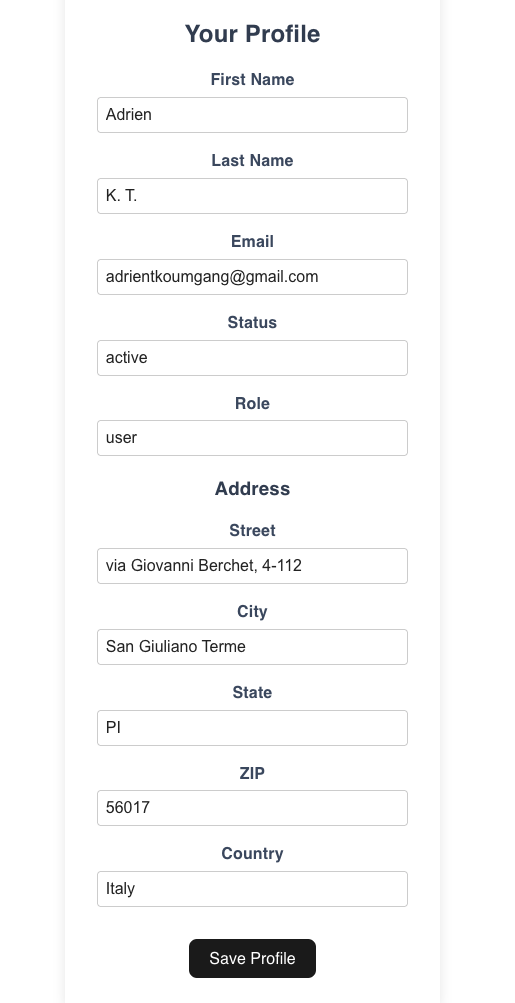
\includegraphics[width=0.8\textwidth]{chapters/chapter_03/page/user/profile-page}
        \caption{User screens: profile page}
        \label{fig:profile-wireframes}
    \end{minipage}
    \hfil
    \begin{minipage}{0.48\linewidth}
        \centering
        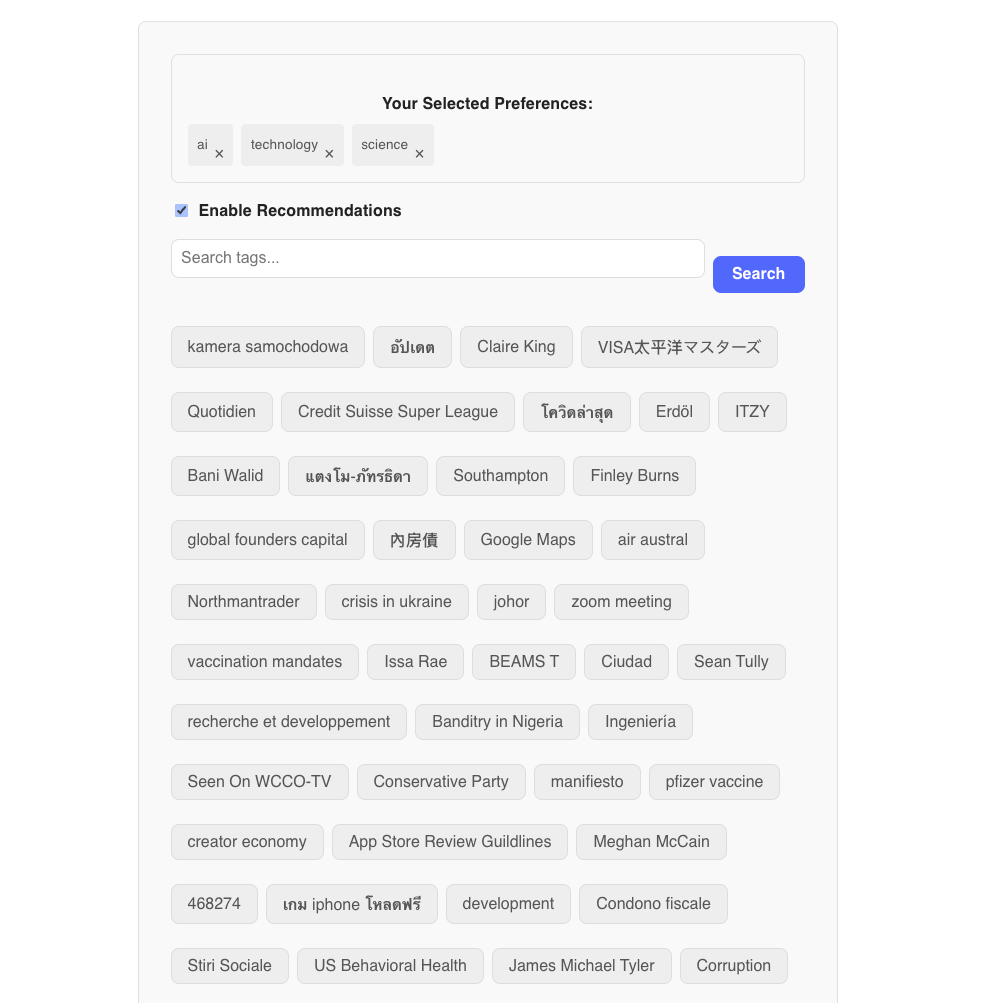
\includegraphics[width=1.2\textwidth]{chapters/chapter_03/page/user/settings-page}
        \caption{User screens: settings page}
        \label{fig:settings-wireframes}
    \end{minipage}
\end{figure}


\begin{figure}[!h]
    \centering
    \begin{minipage}{0.48\linewidth}
        \centering
        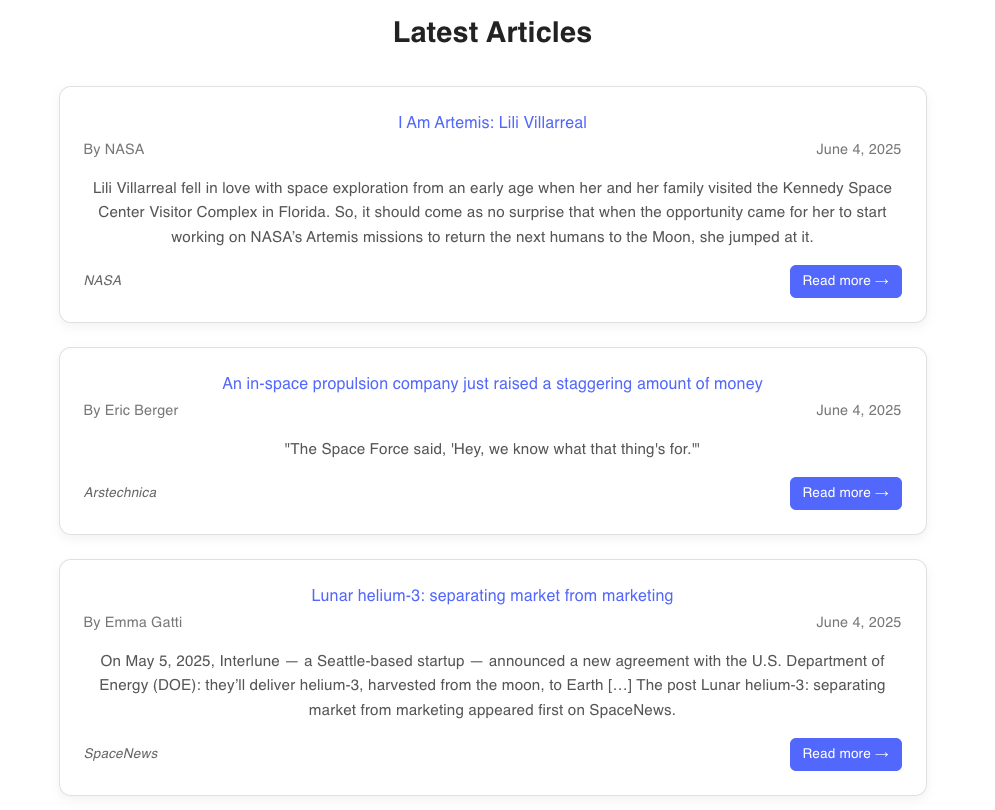
\includegraphics[width=1\textwidth]{chapters/chapter_03/page/user/latest-page}
        \caption{User screens: latest page}
        \label{fig:latest-wireframes}
    \end{minipage}
    \hfil
    \begin{minipage}{0.48\linewidth}
        \centering
        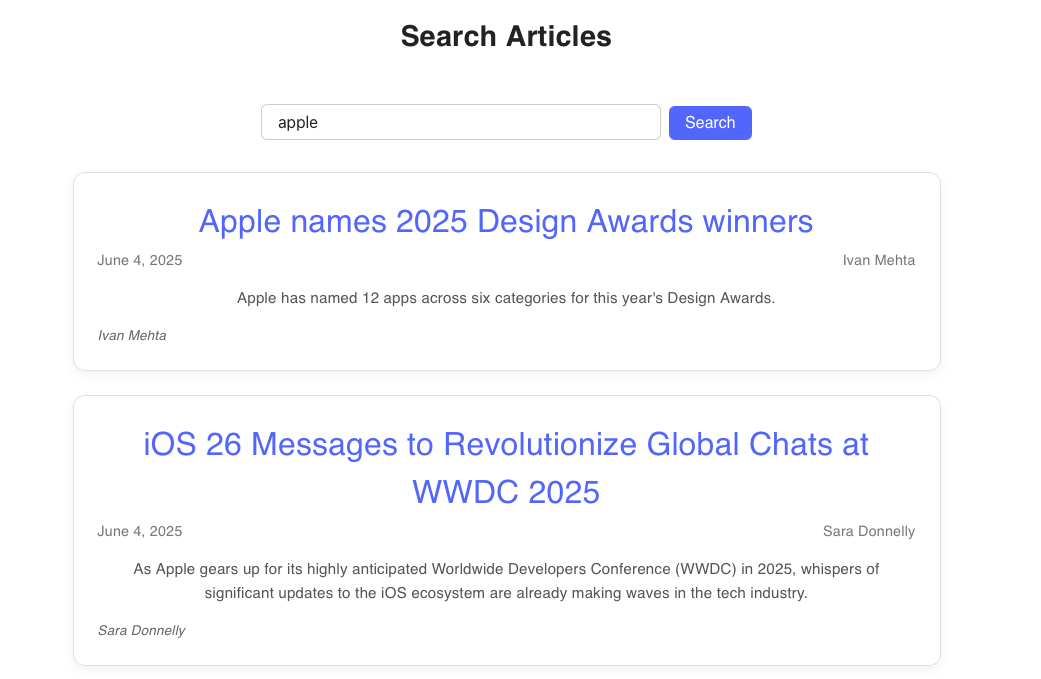
\includegraphics[width=1\textwidth]{chapters/chapter_03/page/user/search-page}
        \caption{User screens: Search page}
        \label{fig:search-wireframes}
    \end{minipage}
\end{figure}


\begin{figure}[!h]
    \centering
    \begin{minipage}{0.48\linewidth}
        \centering
        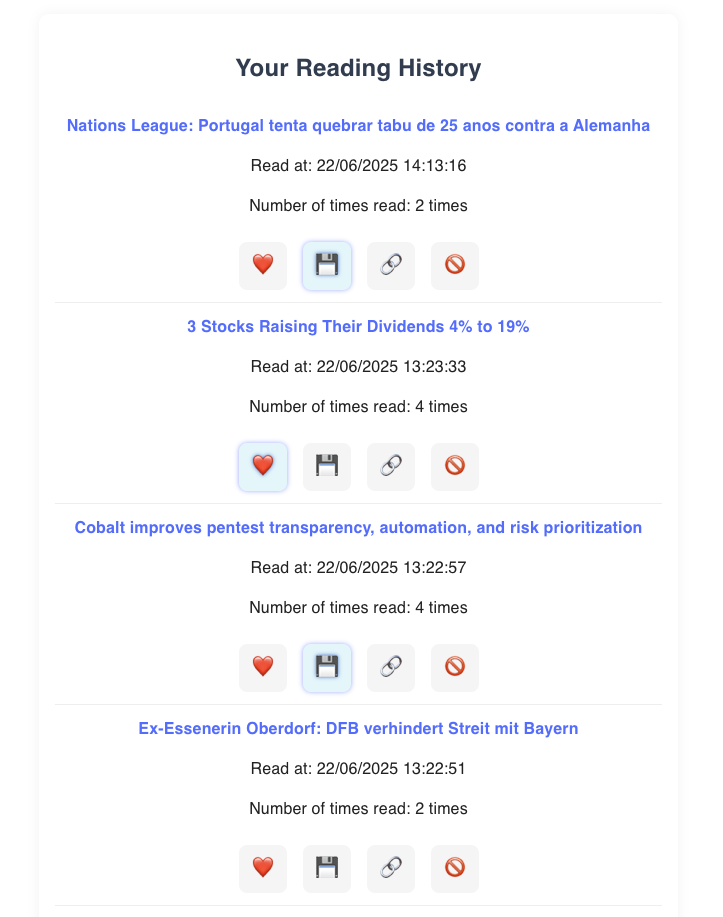
\includegraphics[width=1\textwidth]{chapters/chapter_03/page/user/history-page}
        \caption{User screens: History page}
        \label{fig:history-wireframes}
    \end{minipage}
    \hfil
    \begin{minipage}{0.48\linewidth}
        \centering
        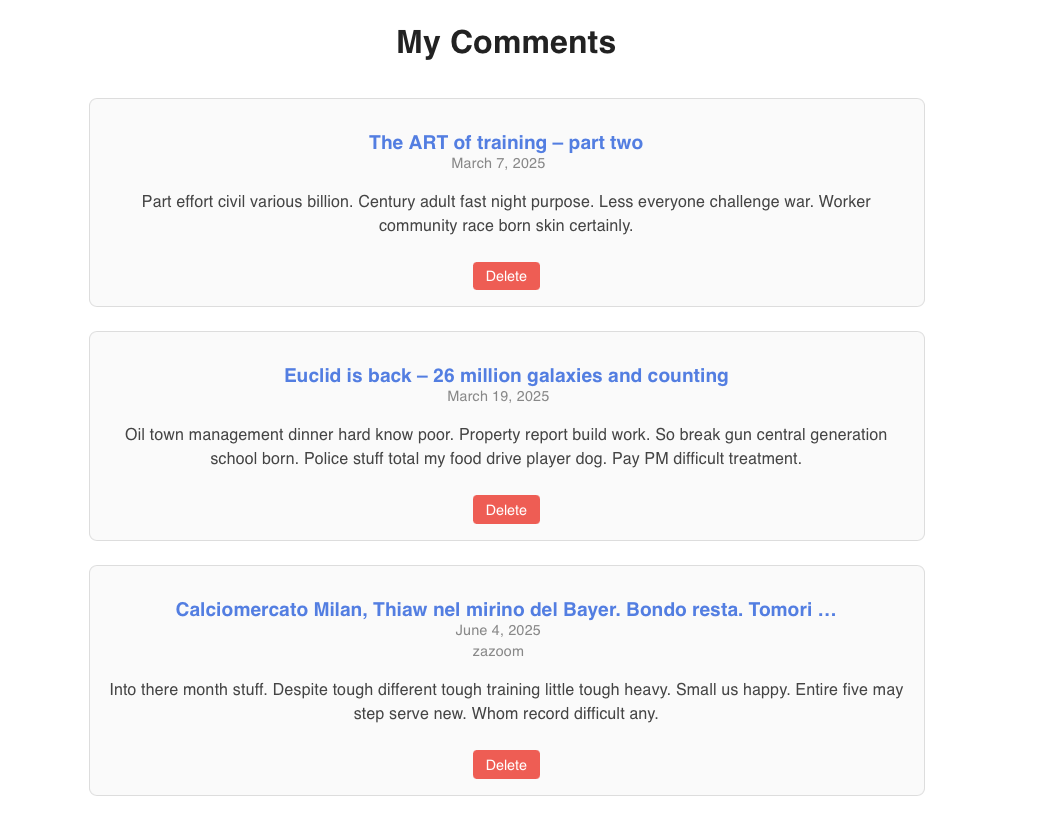
\includegraphics[width=1\textwidth]{chapters/chapter_03/page/user/comments-page}
        \caption{User screens: Comments page}
        \label{fig:comments-wireframes}
    \end{minipage}
\end{figure}



\begin{figure}[!h]
    \centering
    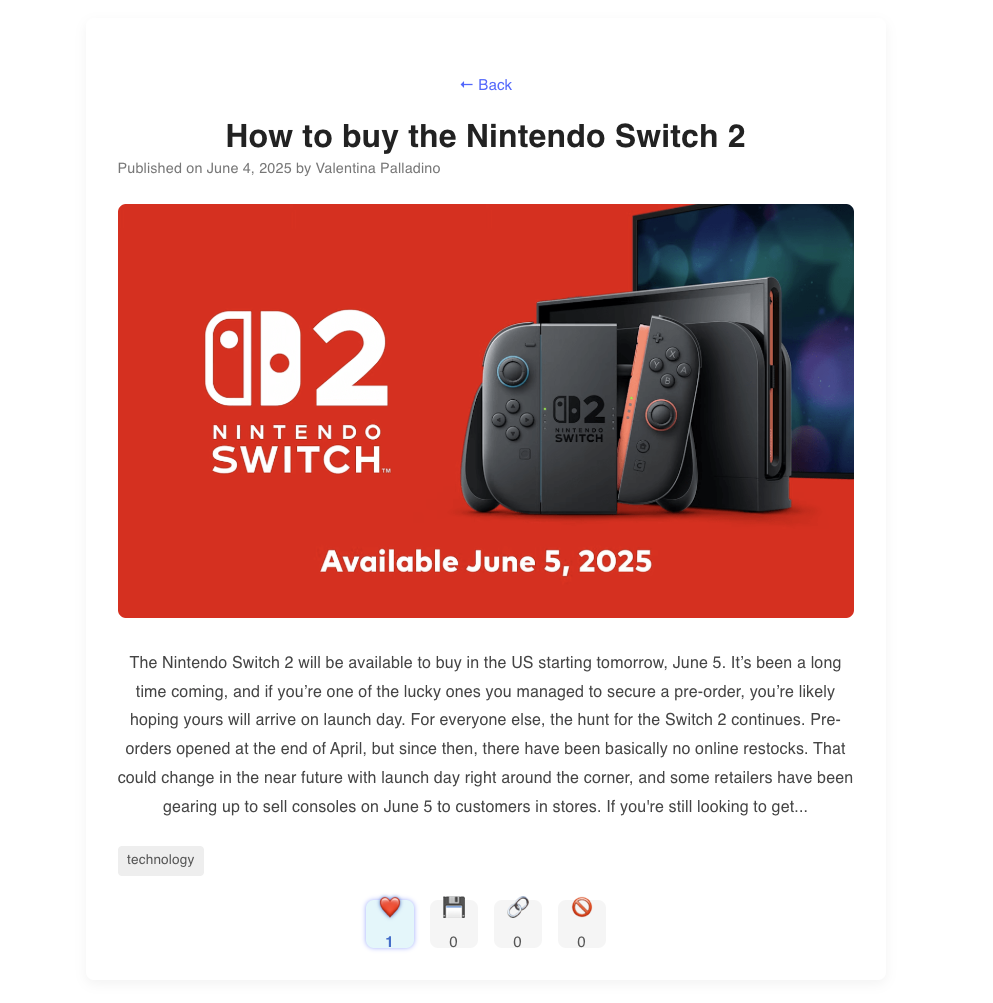
\includegraphics[width=0.7\textwidth]{chapters/chapter_03/page/user/article-details-page}
    \caption{User screens: articles details page}
    \label{fig:articles-details-wireframes}
\end{figure}


\subsection{Admin Screens}\label{subsec:admin-screens}

\begin{figure}[!h]
    \centering
    \begin{minipage}{0.48\linewidth}
        \centering
        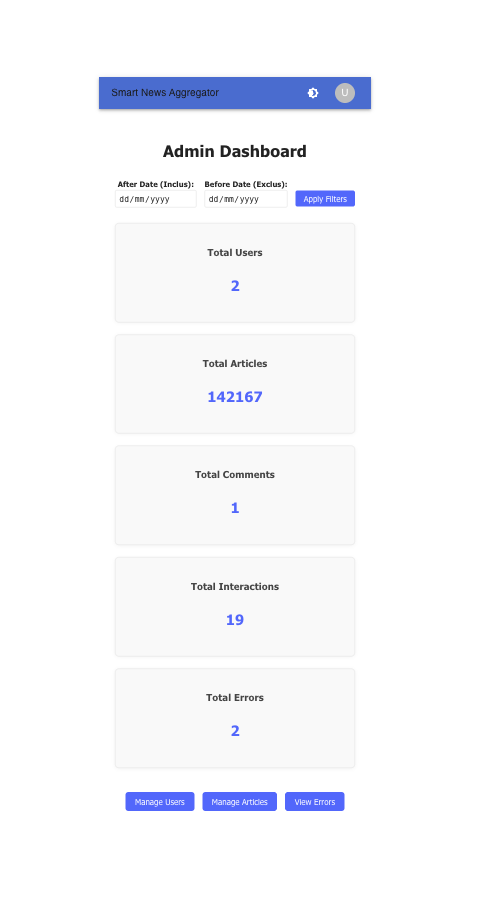
\includegraphics[width=1\textwidth]{chapters/chapter_03/page/admin/admin-dashboard-page}
        \caption{Admin screens: admin dashboard page}
        \label{fig:admin-dashboard-wireframes}
    \end{minipage}
    \hfil
    \begin{minipage}{0.48\linewidth}
        \centering
        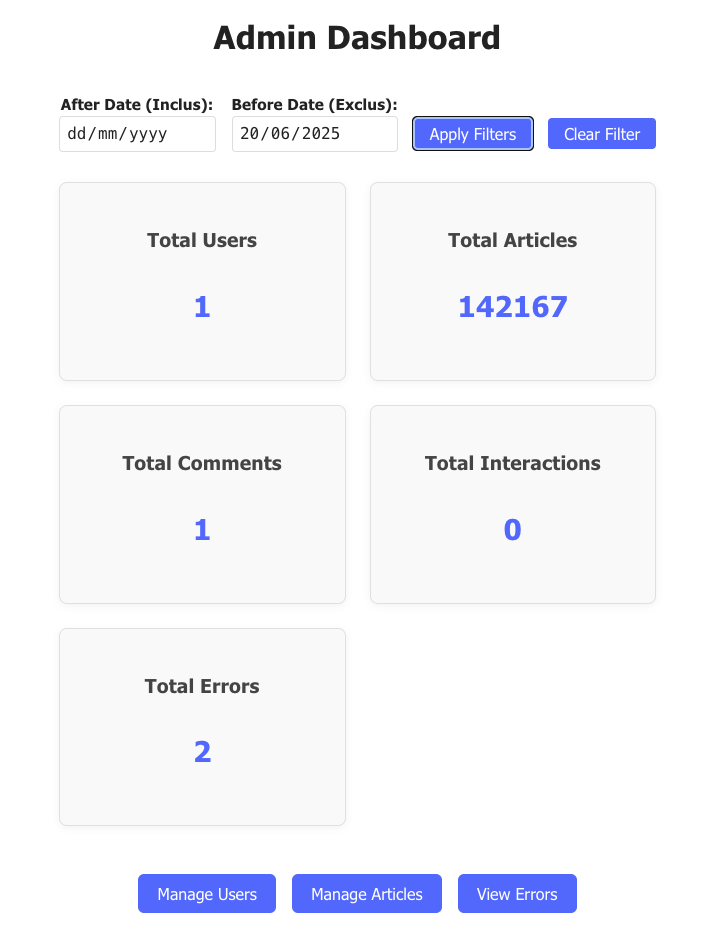
\includegraphics[width=1\textwidth]{chapters/chapter_03/page/admin/admin-dashboard-page-2}
        \caption{Admin screens: admin dashboard page}
        \label{fig:admin-dashboard-2-wireframes}
    \end{minipage}
\end{figure}


\begin{figure}[!h]
    \centering
    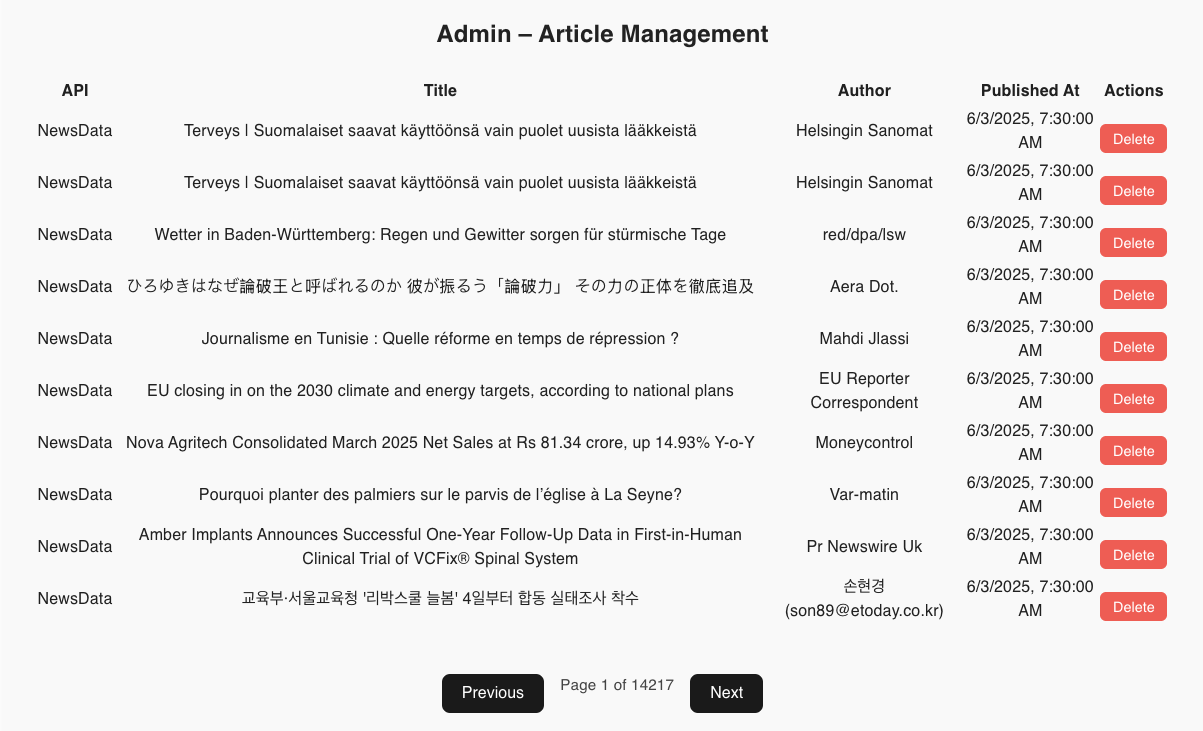
\includegraphics[width=0.7\textwidth]{chapters/chapter_03/page/admin/admin-articles-page}
    \caption{Admin screens: admin articles page}
    \label{fig:admin-articles-wireframes}
\end{figure}

\begin{figure}[!h]
    \centering
    \begin{minipage}{0.48\linewidth}
        \centering
        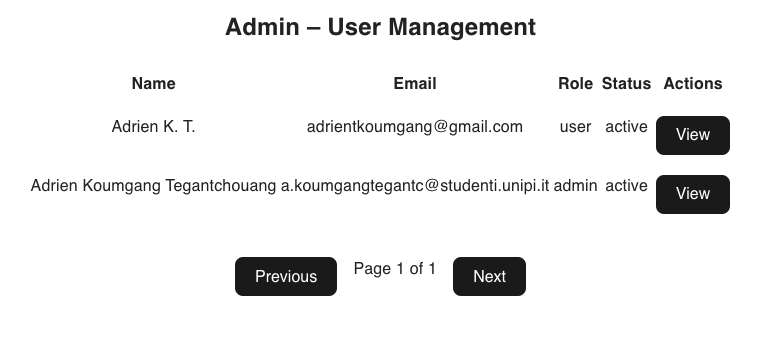
\includegraphics[width=1\textwidth]{chapters/chapter_03/page/admin/admin-users-page}
        \caption{Admin screens: admin users page}
        \label{fig:admin-users-wireframes}
    \end{minipage}
    \hfil
    \begin{minipage}{0.48\linewidth}
        \centering
        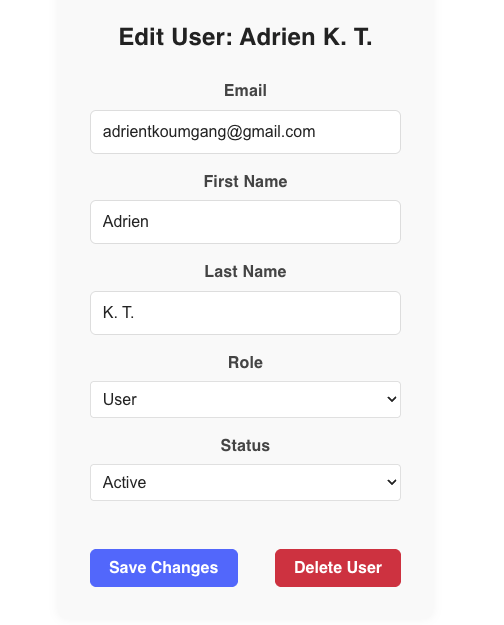
\includegraphics[width=1\textwidth]{chapters/chapter_03/page/admin/admin-user-details-page}
        \caption{Admin screens: admin user details page}
        \label{fig:admin-user-details-wireframes}
    \end{minipage}
\end{figure}


\begin{figure}[!h]
    \centering
    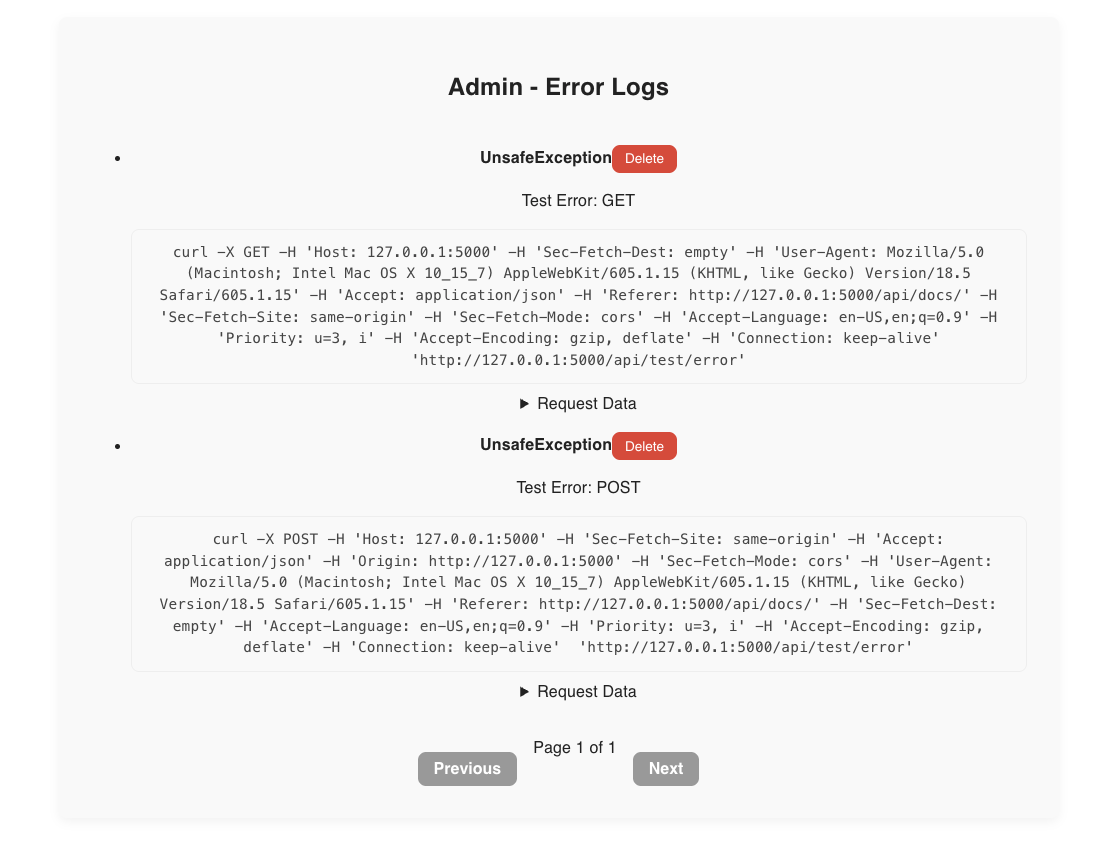
\includegraphics[width=0.7\textwidth]{chapters/chapter_03/page/admin/admin-error-logs-page}
    \caption{Admin screens: admin error logs page}
    \label{fig:admin-error-logs-wireframes}
\end{figure}





% Data Modeling
    %! Author = adrienkoumgangtegantchouang
%! Date = 09/06/25

\chapter{Data Modeling}\label{ch:data-modeling}

In designing the project, I employed a \textbf{hybrid data modeling strategy} that combines both \textbf{relational}
and \textbf{NoSQL (document-based and key-value)} approaches to balance data consistency, flexibility, and performance at scale.

\section{Databases Technologies Used}\label{sec:databases-technologies-used}

\begin{itemize}
    \item \textbf{MongoDB (Document Database, version 6.0)}: Used for modeling core entities like user, articles, comments, user interactions and logs.
    \item \textbf{Redis (Key-Value Store, version 7.0)}: Used for caching.
\end{itemize}

\section{MongoDB Data Models}\label{sec:mongodb-data-models}

MongoDB is used as the primary \textbf{document database} to store structured yet flexible data such as users, articles, comment, interactions and errors server.
Its schema-less nature and native support for nested documents make it suitable for dynamic content and high-volume ingestion\cite{pydantic}.

MongoDB stores structured documents for core domain entities.
Each entity is represented as a collection with JSON-like documents.
The key collections are:

\subsection{Users collection}\label{subsec:users-collection}


\begin{lstlisting}[language=json,label={lst:users-collection-json-example}]
{
  "_id": {
    "$oid": "683c758466d99ae51f0508d4"
  },
  "created_at": {
    "$date": "2025-06-01T15:45:08.196Z"
  },
  "updated_at": {
    "$date": "2025-06-21T03:25:04.294Z"
  },
  "firstname": "Adrien",
  "lastname": "K. T.",
  "email": "adrientkoumgang@gmail.com",
  "password": "$2b$12$tSDjoy8m4IMBS6T/As5zveHctHxvkUmaslrONegD4kRPpkgPARlJK",
  "account": {
    "status": "active",
    "role": "user"
  },
  "password_history": [
    {
      "password": "$2b$12$guC9jr36y2MEW50le9S4wOdKbZsVnmRrXAvk5S2IMJ4QSkJSTaG5e",
      "created_at": {
        "$date": "2025-06-01T15:45:08.196Z"
      }
    },
    {
      "password": "$2b$12$tSDjoy8m4IMBS6T/As5zveHctHxvkUmaslrONegD4kRPpkgPARlJK",
      "created_at": {
        "$date": "2025-06-05T20:51:45.379Z"
      }
    }
  ],
  "preferences_enable": true,
  "preferences": [
    "ai",
    "technology",
    "science"
  ],
  "address": {
    "street": "via Giovanni Berchet, 4-112",
    "city": "San Giuliano Terme",
    "state": "PI",
    "zip": "56017",
    "country": "Italy"
  }
}
\end{lstlisting}

\textbf{Indexes:}

\begin{enumerate}
  \item $\{ email: 1 \}$ (Unique) : Email indexes enables fast login lookups and registration check.
  \item $\{ preferences: 1 \}$ (Multikey) : Preferences index accelerates personalized feed generation.
\end{enumerate}


\subsection{Article log requests collection}\label{subsec:article-log-requests-collection}

\begin{lstlisting}[language=json,label={lst:article-log-requests-collection-json-example}]
{
  "_id": {
    "$oid": "68402a68a26f0389a8c4ed9e"
  },
  "created_at": {
    "$date": "2025-06-04T11:13:44.758Z"
  },
  "updated_at": {
    "$date": "2025-06-04T11:13:44.758Z"
  },
  "source": "CurrentsAPI",
  "url": "https://api.currentsapi.services/v1/latest-news",
  "request": {
    "url": "https://api.currentsapi.services/v1/latest-news",
    "headers": {
      "Authorization": "97ueDaaD6tgJItwJhzKGqd1FYoXm3xZ6H3-lAxKXloZmRYdm"
    },
    "params": {}
  },
  "response": {
    "status_code": 200,
    "returned": 30
  },
  "fetched_count": 30
}
\end{lstlisting}

\textbf{Indexes:}

\begin{enumerate}
  \item $\{ created\_at: -1, source: 1 \}$ (Compound): optimize time-based queries filtered by API source.
    Monitoring recent API fetch operations by provider.
  \item $\{ response.status\_code: -1 \}$ : quickly identify failed requests for error monitoring and alerting.
\end{enumerate}


\subsection{Articles collection}\label{subsec:articles-collection}


\begin{lstlisting}[language=json,label={lst:articles-collection-json-example}]
{
  "_id": {
    "$oid": "6840d72e34b1dd6ef4c87b05"
  },
  "created_at": {
    "$date": "2025-06-04T23:30:53.992Z"
  },
  "updated_at": {
    "$date": "2025-06-04T23:30:53.992Z"
  },
  "extern_id": "b13b8ed2543f2ca7e1874fc2e63282e0",
  "extern_api": "NewsData",
  "title": "EU closing in on the 2030 climate and energy targets, according to national plans",
  "description": "EU member states have significantly closed the gap to achieving the 2030 energy and climate targets, according to the European Commission's assessment of the National Energy and Climate Plans (NECPs). EU countries have substantially improved their plans following Commission recommendations in December 2023. As a result, the EU is closing in collectively on a 55% reduction in greenhouse gas (GHG) emissions, as committed [...]",
  "content": "ONLY AVAILABLE IN PAID PLANS",
  "url": "https://www.eureporter.co/environment/2025/06/03/eu-closing-in-on-the-2030-climate-and-energy-targets-according-to-national-plans/",
  "author": {
    "name": "EU Reporter Correspondent"
  },
  "source": {
    "name": "Eureporter Co",
    "url": "https://www.eureporter.co"
  },
  "published_at": "2025-06-03 07:30:00",
  "language": "english",
  "country": "united kingdom",
  "tags": [
    "environment",
    "full-image",
    "climate-neutral economy",
    "climate change",
    "featured"
  ]
}
\end{lstlisting}

\textbf{Indexes:}

\begin{enumerate}
  \item $\{ external\_api: 1, external\_id: 1, title: 1 \}$ (Compound, Unique) : External ID index prevents duplicates articles.
  \item $\{ published\_at: -1 \}$ : Date indexes support chronological queries
  \item $\{ tags: 1, published\_at: -1 \}$ (Compound): this compound index optimizes feed generation
  \item $\{ tags: 1 \}$: for search all possible tags in all articles
  \item $\{ title: "text", description: "text" \}$ (Text): Text index enables full-text search.
  (Creation failure due to invalid characters such as Japanese and other non-Latin characters.)
\end{enumerate}

\subsection{Comments collection}\label{subsec:comments-collection}

\begin{lstlisting}[language=json,label={lst:comments-collection-json-example}]
{
  "_id": {
    "$oid": "684d39437a0814577744e01d"
  },
  "created_at": {
    "$date": "2025-06-14T08:26:06.817Z"
  },
  "updated_at": {
    "$date": "2025-06-14T08:26:06.818Z"
  },
  "user_id": "683c758466d99ae51f0508d4",
  "article_id": "6840dbaa2c0129e299fbd9db",
  "content": "My first comment"
}
\end{lstlisting}

\textbf{Indexes:}

\begin{enumerate}
  \item $\{ article\_id: 1, created\_at: -1 \}$ (Compound): this index optimizes comment threading.
  \item $\{ user\_id: 1 \}$: User index supports profile activity views
  \item $\{ user\_id: 1, created\_at: -1 \}$ (Compound): User index supports profile activity views
  \item $\{ comment\_fk: 1, created\_at: -1 \}$ (Compound): this index enables efficient nested comment retrieval
\end{enumerate}

\subsection{User Interactions collection}\label{subsec:user-interactions-collection}

\begin{lstlisting}[language=json,label={lst:articles-users-interactions-collection-json-example}]
{
  "_id": {
    "$oid": "6855a9d4ecbd85c7cbce08e2"
  },
  "article_id": "6840db802c0129e299fbbe29",
  "user_id": "683c758466d99ae51f0508d4",
  "article_title": "Apple names 2025 Design Awards winners",
  "level_interaction": "article",
  "liked": true,
  "read_at": {
    "$date": "2025-06-20T18:35:00.451Z"
  },
  "saved": true,
  "shared": false,
  "time_spent": 2,
  "updated_at": {
    "$date": "2025-06-20T18:35:00.451Z"
  },
  "report": false
}
\end{lstlisting}

\textbf{Indexes:}

\begin{enumerate}
  \item $\{ user\_id: 1,  read\_at: -1\}$ (Compound): this index powers reading history
  \item $\{ article\_id: 1 \}$ : this index supports engagement analytics
  \item $\{ article\_id: 1,  updated\_at: -1\}$ (Compound): this index powers reading article stats
\end{enumerate}

\subsection{Server Error Logs collection}\label{subsec:server-error-logs-collection}

\begin{lstlisting}[language=json,label={lst:server-logs-collection-json-example}]
{
  "_id": {
    "$oid": "684241a852621fd670c36a1c"
  },
  "created_at": {
    "$date": "2025-06-06T01:17:05.512Z"
  },
  "updated_at": {
    "$date": "2025-06-06T01:17:05.512Z"
  },
  "request_data": {
    "url": "http://127.0.0.1:5000/api/test/error",
    "method": "POST",
    "body": {},
    "args": {},
    "headers": {
      "Host": "127.0.0.1:5000",
      "Sec-Fetch-Site": "same-origin",
      "Accept": "application/json",
      "Origin": "http://127.0.0.1:5000",
      "Sec-Fetch-Mode": "cors",
      "User-Agent": "Mozilla/5.0 (Macintosh; Intel Mac OS X 10_15_7) AppleWebKit/605.1.15 (KHTML, like Gecko) Version/18.5 Safari/605.1.15",
      "Referer": "http://127.0.0.1:5000/api/docs/",
      "Sec-Fetch-Dest": "empty",
      "Content-Length": "0",
      "Accept-Language": "en-US,en;q=0.9",
      "Priority": "u=3, i",
      "Accept-Encoding": "gzip, deflate",
      "Connection": "keep-alive"
    },
    "form": {}
  },
  "curl": "curl -X POST -H 'Host: 127.0.0.1:5000' -H 'Sec-Fetch-Site: same-origin' -H 'Accept: application/json' -H 'Origin: http://127.0.0.1:5000' -H 'Sec-Fetch-Mode: cors' -H 'User-Agent: Mozilla/5.0 (Macintosh; Intel Mac OS X 10_15_7) AppleWebKit/605.1.15 (KHTML, like Gecko) Version/18.5 Safari/605.1.15' -H 'Referer: http://127.0.0.1:5000/api/docs/' -H 'Sec-Fetch-Dest: empty' -H 'Accept-Language: en-US,en;q=0.9' -H 'Priority: u=3, i' -H 'Accept-Encoding: gzip, deflate' -H 'Connection: keep-alive'  'http://127.0.0.1:5000/api/test/error'",
  "exception_name": "UnsafeException",
  "exception_message": "Test Error: POST"
}
\end{lstlisting}

\textbf{Indexes:}

\begin{enumerate}
  \item $\{ created\_at \}$ : this index support log rotation
\end{enumerate}

\section{Redis Data Structures}\label{sec:redis-data-structures}

\subsection{Article Caching}\label{subsec:article-caching}

When an article appears in a user's News Feed, there's a probability that the user will want to read it, so the article is fully cached for quick access.
This with a ttl of 10 minutes.

\subsection{User caching}\label{subsec:user-caching}

The user comes fully cached for fast access especially for his reading preferences.
This with an infinite ttl.







% Data Ingestion and Intetration
    %! Author = adrienkoumgangtegantchouang
%! Date = 09/06/25

\chapter{Data Ingestion and Integration}\label{ch:data-ingestion-and-integration}


The \textbf{Smart News Aggregator} relies on real-time and scheduled data ingestion from multiple external news APIs.
This chapter details the data pipeline architecture, API integration strategies, preprocessing steps,
and error handling mechanisms to ensure a consistent and reliable flow of news articles into the system.


\section{External API Integration}\label{sec:external-api-integration}


The system integrates with the following news providers:

\begin{table}[h!]
  \centering
  \begin{tabular}{|l|l|l|c|}
    \hline
    API & Description & Rate Limits & Data Format \\
    \hline
    \textbf{MediaStack} & News articles from 7,500+ sources & 500 requests/month & JSON \\
    \textbf{CurrentsApi} & - & x requests/month & JSON \\
    \textbf{Gnews} & - & x requests/month & JSON \\
    \textbf{MarketAux} & - & x requests/month & JSON \\
    \textbf{NYTimes} & Premium news content & 4000 requests/month & JSON \\
    \textbf{News Api} & - & x requests/month & JSON \\
    \textbf{News Data} & Global news coverage & 100 requests/month & JSON \\
    \textbf{Space Flight News Api} & - & x requests/month & JSON \\
    \textbf{The Guardian} & High-quality journalism & 5,000 requests/month & JSON \\
    \hline
  \end{tabular}
  \caption{External Api Integration}
  \label{tab:external-api-integration}
\end{table}


Each API uses API keys stored securely in environment variables.
Scheduled cron job triggers API calls every monday at 00:00.
Requests are made via requests.
Response Handling: On success, Normalize and store in MongoDB. On failure, Log error, retry with backoff (max 3 attempts).


\section{Data Processing}\label{sec:data-processing}


\subsection{Data Validation}\label{subsec:data-validation}

\begin{itemize}
    \item \textbf{Duplicate Detection}: checks $external id$ and mongodb index $\{ external\_api: 1, external\_id: 1, title: 1 \}$ (Compound, Unique)
    \item \textbf{Schema Validation}: Ensures required field ($title$, $url$ $published\_at$)
\end{itemize}

\subsection{Data Normalization}\label{subsec:data-normalization}

\textbf{Standardized Schema}


\section{Error Handling and Logging}\label{sec:error-handling-and-logging}


For error type is \textbf{rate limit exceeded}, retry the next week.
For \textbf{network failure}, exponential backoff (max 3 retries).
And for \textbf{malformed data}, skips invalid entries.





% Backend Implementation
    %! Author = adrienkoumgangtegantchouang
%! Date = 09/06/25


\chapter{Backend Implementation}\label{ch:backend-implementation}


This backend of the \textbf{Smart News Aggregator} is built using \textbf{Flask} (Python) with \textbf{Flask-RESTX} for API development.


\section{System Architecture}\label{sec:system-architecture}


\subsection{Key Components}\label{subsec:backend-key-components}

\begin{tabular}{lll}
  \toprule
  Component & Technology & Purpose \\
  \midrule
  API Server & Flask\cite{flask, flaskrestx} + Gunicor & HTTP request handling \\
  Auth & JWT(RS256)\cite{jwt}  & User authentication \\
  Caching & Redis & Session/store hot data \\
  Asybc Tasks & Flask Cron & Background jobs (API fetching) \\
  Docs & Swagger UI\cite{swagger} & Interactive API documentation \\
  \bottomrule
\end{tabular}


\section{API Endpoints}\label{sec:api-endpoints}


\subsection{Authentication}\label{subsec:authentication}

\begin{tabularx}{\textwidth}{lcX}
  \toprule
  Endpoint & Method & Description \\
  \midrule
  $/auth/register$ & POST & User registration \\
  $/auth/login$ & POST  & JWT token generation \\
  $/auth/login-alt$ & POST & JWT token generation without password validation \\
  $/auth/change\_password$ & POST & Update user password \\
  $/auth/me$ & GET & Get current user information like email, name, status, role \\
  \bottomrule
\end{tabularx}

\begin{figure}[!h]
    \centering
    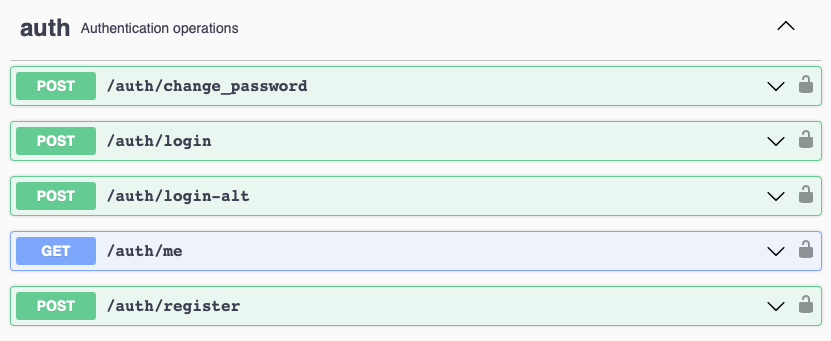
\includegraphics[width=1\textwidth]{chapters/chapter_06/authentication-operations}
    \caption{API Endpoint: Authentication endpoint}
    \label{fig:api-authentication-endpoint}
\end{figure}


\subsection{User Management}\label{subsec:user-management}


\begin{tabularx}{\textwidth}{lcX}
  \toprule
  Endpoint & Method & Description \\
  \midrule
  $/user/article/preference$ & POST & Add article preference tags for current user \\
  $/user/article/preference$ & GET & Get article preference tags for current user \\
  $/user/me$ & POST & Update current user information \\
  $/user/me$ & GET & Get current user information \\
  \bottomrule
\end{tabularx}

\begin{figure}[!h]
    \centering
    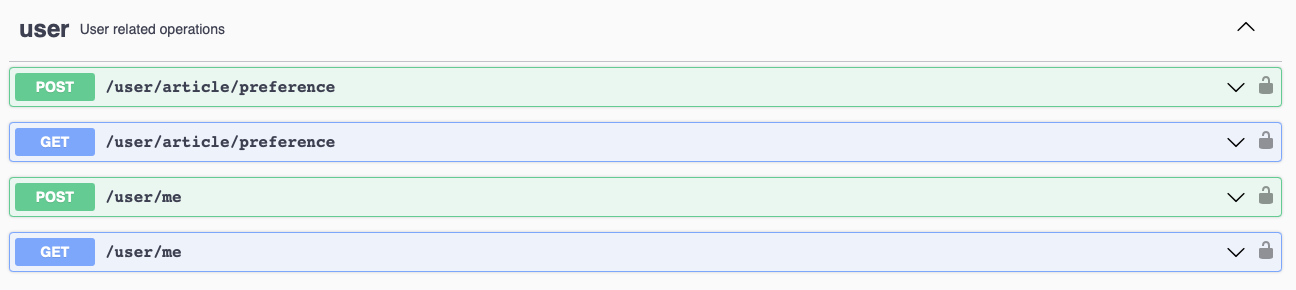
\includegraphics[width=1\textwidth]{chapters/chapter_06/user-operations}
    \caption{API Endpoint: User endpoint}
    \label{fig:api-user-endpoint}
\end{figure}


\subsection{Article Management}\label{subsec:article-management}

\begin{tabularx}{\textwidth}{XcX}
  \toprule
  Endpoint & Method & Description \\
  \midrule
  $/article/comment/me$ & GET & List of comment make by current user \\
  $/article/history$ & GET & List of read articles \\
  $/article/latest$ & GET & List of all articles order by recent published \\
  $/article/search$ & GET & List of article where title or description content query \\
  $/article/tags$ & POST & - \\
  $/article/tags$ & GET & - \\
  $/article/\{article\_id\}$ & GET & Get all article data \\
  $/article/\{article\_id\}/comment$ & POST & Add comment on article \\
  $/article/\{article\_id\}/comment$ & GET & List of comment for this specific article \\
  $/article/\{article\_id\}/comment/$ $\{comment\_id\}$ & GET & Get all comment data \\
  $/article/\{article\_id\}/comment/$ $\{comment\_id\}$ & DELETE & Delete specific comment \\
  $/article/\{article\_id\}/comment/$ $\{comment\_id\}/interaction$ & POST & add interaction in this comment \\
  $/article/\{article\_id\}/comment/$ $\{comment\_id\}/interaction$ & GET & Get interaction information in this comment \\
  $/article/\{article\_id\}/interaction$ & POST & Add interaction in this article \\
  $/article/\{article\_id\}/interaction$ & GET & Get article interaction information \\
  $/article/\{article\_id\}/summary$ & GET & Get summable details of this article \\
  \bottomrule
\end{tabularx}


\begin{figure}[!h]
    \centering
    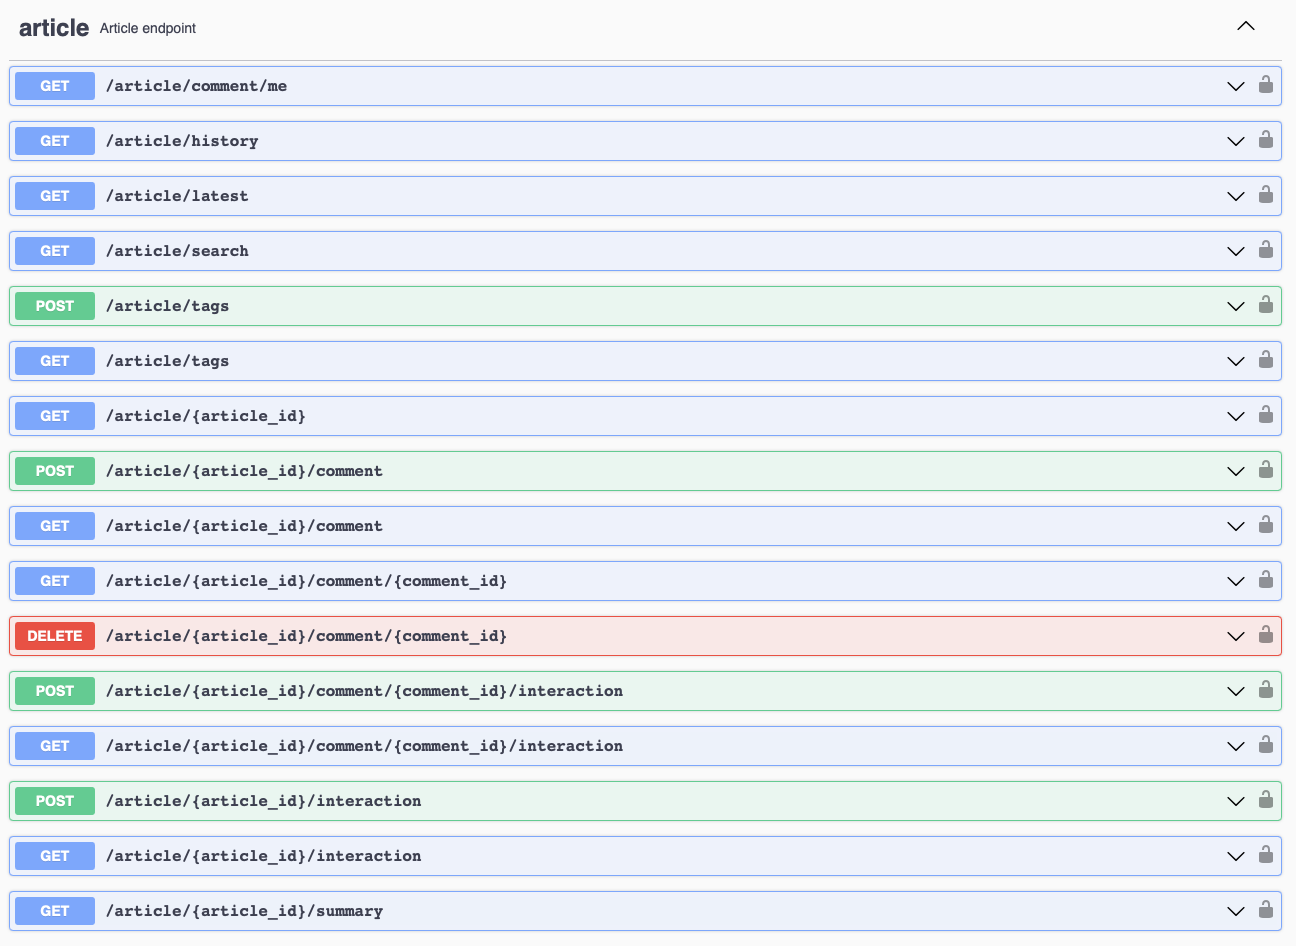
\includegraphics[width=1\textwidth]{chapters/chapter_06/articles-operations}
    \caption{API Endpoint: Articles endpoint}
    \label{fig:api-articles-endpoint}
\end{figure}


\subsection{Administration Management}\label{subsec:admin-management}

\begin{tabularx}{\textwidth}{XcX}
  \toprule
  Endpoint & Method & Description \\
  \midrule
  $/admin/article/\{article\_id\}$ & DELETE & Delete Article \\
  $/admin/articles$ & GET & List of all articles \\
  $/admin/dashboard/errors$ & GET & List of log of errors occur in server during execution \\
  $/admin/dashboard/errors/$ $\{server\_error\_log\_id\}$ & DELETE & delete server error log \\
  $/admin/users$ & GET & List of all users \\
  $/admin/user/\{user\_id\}$ & GET & Get all user data \\
  $/admin/user/\{user\_id\}$ & PUT & Add user \\
  $/admin/user/\{user\_id\}$ & POST & Update user \\
  $/admin/user/\{user\_id\}$ & DELETE & Delete User \\
  $/admin/$ & GET & - \\
  \bottomrule
\end{tabularx}

\begin{figure}[!h]
    \centering
    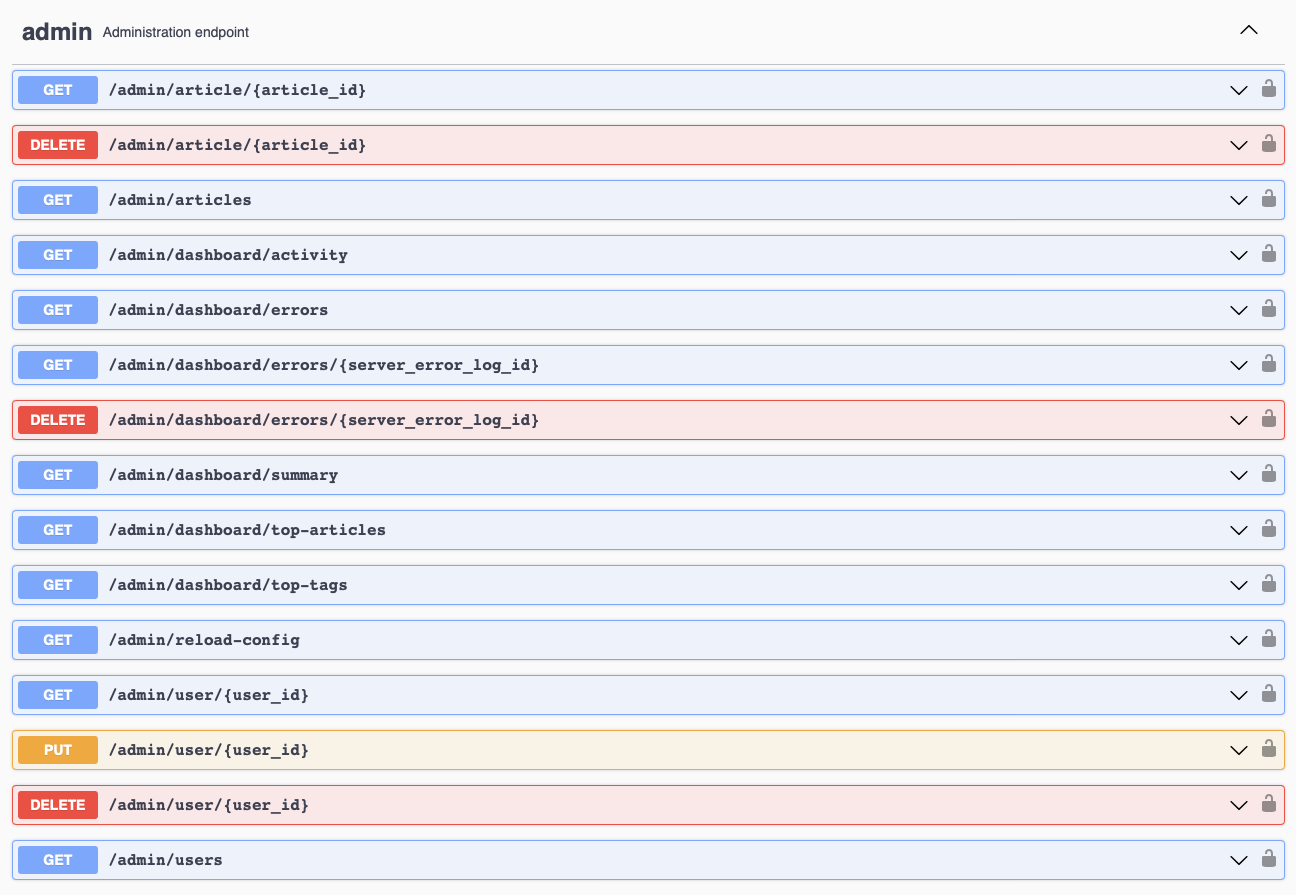
\includegraphics[width=1\textwidth]{chapters/chapter_06/admin-operations}
    \caption{API Endpoint: Admin endpoint}
    \label{fig:api-admin-endpoint}
\end{figure}


\section{Security Implementation}\label{sec:security-implementation}

\subsection{JWT Authentication}\label{subsec:jwt-authentication}

\textbf{Algorithm RS256 (asymmetric)} for token and \textbf{validation middleware}:

\begin{lstlisting}[style=pythonstyle,label={lst:decoration-token-required},caption={Decoration 'Token Required'}]
def token_required(f):
    @wraps(f)
    def decorated(*args, **kwargs):
        token = None

        # Extract token from Authorization header
        auth_header = request.headers.get('Authorization', '')
        if auth_header.startswith("Bearer "):
            token = auth_header.split(" ")[1]

        if not token:
            return {'error': 'Token is missing!'}, 401

        try:
            user = TokenManager.decode_token(token=token)

            if 'admin' in request.url and user.role != 'admin':
                raise UnauthorizedException('You are not authorized to perform this operation')

            g.user = user
        except TokenException as e:
            return {'error': str(e)}, 401

        return f(*args, **kwargs)

    return decorated
\end{lstlisting}

\subsection{Input Validation}\label{subsec:input-validation}

All input data is validated via flask-rest's marshal service, which ensures the integrity of input data.

\begin{lstlisting}[style=pythonstyle,label={lst:input-validation-with-marshal},caption={Input validation with marshal}]
@ns_article.route('/<string:article_id>/interaction')
@ns_article.param('article_id', 'The article ID')
class ArticleInteractionResource(Resource):
    @token_required
    @ns_article.expect(ArticleInteractionType.to_model(name_space=ns_article))
    @ns_article.marshal_with(Model.get_message_response_model(name_space=ns_article))
    def post(self, article_id):
        user_token: UserToken = g.user

        data = request.get_json()
        interaction = ArticleInteractionType(**data)
        result = UserArticleInteractionModel.update_interaction(user_token, interaction=interaction, article_id=article_id)

        if result:
            return {"success": True, "message": "Interaction updated"}
        return {"success": False, "message": "Interaction could not be updated"}
\end{lstlisting}


\section{Performance Optimizations}\label{sec:performance-optimizations}

\subsection{Caching Strategies}\label{subsec:caching-strategies}

\begin{tabularx}{\textwidth}{lXl}
  \toprule
  Cache Key & Data & TTL \\
  \midrule
  $user:\<user\_id\>$ & Full user json & - \\
  $article:\<article\_id\>$ & - & - \\
  $article:last:count$ & all last articles count & - \\
  $article:last:\<user\_id\>:count$ & all last articles count with user preferences & - \\
  $article:last:\<page\>:\<limit\>$ & full list last articles json by page and limit & - \\
  $article:all:count$ & all articles count & - \\
  $article:all:\<page\>:\<limit\>$ & full list articles json by page and limit & - \\
  $comment:all:\<filter\>:\<page\>:\<limit\>$ & full list comment by article, page and limit  & - \\
  \bottomrule
\end{tabularx}

\subsection{Async Task Processing}\label{subsec:async-task-processing}

When a user accesses a list of items via services such as latest, history, each item in the list is cached.

\begin{lstlisting}[style=pythonstyle,label={lst:async-cache-article},caption={Async Cache Article}]
class ArticleModel(ArticleSummaryModel):
    @classmethod
    def _cache_articles(cls, user_token: UserToken, articles: list):
        for article in articles:
            _ = cls.get(user_token, str(article.article_id))

    @classmethod
    def cache_articles(cls, user_token: UserToken, articles: list):
        thread = Thread(target=cls._cache_articles, args=(user_token, articles,))
        thread.daemon = True
        thread.start()
\end{lstlisting}


\section{API Documentation}\label{sec:api-documentation}

My api's documentation is auto-generated using flask-restx namesapces and swagger accessible via swagger ui via endpoint /api/docs.

\begin{lstlisting}[style=pythonstyle,label={lst:api-documentation-article-summary},caption={Api Docuentation Article Summary}]
class ArticleSummaryModel(MongoDBBaseModel):
    @staticmethod
    def to_model(name_space: Namespace):
        return name_space.model('ArticleSummaryModel', {
            'article_id': fields.String(required=False),
            'extern_id': fields.String(required=False),
            'extern_api': fields.String(required=True),
            'title': fields.String(required=True),
            'description': fields.String(required=True),
            'author': fields.Nested(ArticleSourceModel.to_model(name_space)),
            'source': fields.Nested(ArticleSourceModel.to_model(name_space)),
            'image_url': fields.String(required=True),
            'published_at': fields.String(required=True),
            'tags': fields.List(fields.String, description="List of tags"),
            'current_user_interaction': fields.Nested(ArticleInteractionStatus.to_model(name_space)),
            'total_user_interaction': fields.Nested(ArticleInteractionStats.to_model(name_space)),
        })

    @staticmethod
    def to_model_list(name_space: Namespace):
        return name_space.model('ArticleSummaryModelList', {
            'articles': fields.List(fields.Nested(ArticleSummaryModel.to_model(name_space)),),
            'total': fields.Integer,
            'page': fields.Integer,
            'limit': fields.Integer,
            'pageCount': fields.Integer,
        })
\end{lstlisting}








% Advanced Aggregations and Analytics
    %! Author = adrienkoumgangtegantchouang
%! Date = 09/06/25

\chapter{Advanced Aggregations and Analytics}\label{ch:advanced-aggregations-and-analytics}


\section{MongoDB Aggregation Framework}\label{sec:mongodb-aggregation-framework}


\subsection{Key Aggregation Concepts}\label{subsec:key-aggregation-concepts}

\begin{itemize}
    \item \textbf{Pipeline Stages}: Filter ($\$match$), Group ($\$group$), Sort ($\$sort$), Project ($\$project$)
    \item \textbf{Operators}: $\$sum$, $\$avg$, $\$max$, $\$arrayElementAt$, $\$cond$
    \item \textbf{Performance}: Uses indexes, optimized for large datasets
\end{itemize}


\subsection{Pipeline: All tags}\label{subsec:pipeline:-all-tags}

\begin{lstlisting}[style=pythonstyle,label={lst:pipeline:-all-tags},caption={Pipeline All Tags}]
class ArticleModel(ArticleSummaryModel):
    @classmethod
    def get_all_tags(cls, user_token, search: str = None):
        tags = cls._get_all_tags()
        if tags:
            return tags

        api_logger = ApiLogger(f"[MONGODB] [ARTICLE TAGS] [GET ALL] : search = {search}")
        if search:
            pipeline = [
                {"$unwind": "$tags"},
                {"$match": {"tags": {"$regex": f"^{search}", "$options": "i"}}},
                {"$group": {"_id": None, "matchedTags": {"$addToSet": "$tags"}}},
                {"$project": {"_id": 0, "matchedTags": 1}}
            ]
        else:
            pipeline = [
                {"$unwind": "$tags"},
                {"$group": {"_id": None, "matchedTags": {"$addToSet": "$tags"}}},
                {"$project": {"_id": 0, "matchedTags": 1}}
            ]

        with MONGO_QUERY_TIME.time():
            data = cls.collection().aggregate(pipeline)

        result = list(data)
        tags = result[0]['matchedTags'] if result else []

        api_logger.print_log()

        cls._cache_all_tags(tags)

        return tags
\end{lstlisting}


\subsection{Pipeline: Search Articles}\label{subsec:pipeline:-search-articles}

\begin{lstlisting}[style=pythonstyle,label={lst:pipeline-search-articles},caption={Pipeline search articles}]
class ArticleSearchModel(DataBaseModel):
    @classmethod
    def search_articles(cls, user_token: UserToken, query: str, page: int = 1, limit: int = 10):
        if not query:
            return ArticleModel.last_articles(user_token, page=page, limit=limit)

        api_logger = ApiLogger(f"[MONGODB] [ARTICLE LATEST] [GET] : query={query}, page={page} and limit={limit}")

        pipeline = [
            {
                "$match": {
                    "$text": {
                        "$search": query,
                        # "$language": "english"
                    }
                }
            },
            {
                "$project": {
                    'article_id': '$_id',
                    'extern_api': 1,
                    'extern_id': 1,
                    "title": 1,
                    "description": 1,
                    'source': 1,
                    'author': 1,
                    "score": {"$meta": "textScore"},
                    "published_at": 1
                }
            },
            {
                "$sort": {"score": -1, "published_at": -1}  # Relevance + recency
            },
            {
                "$skip": (page - 1) * limit
            },
            {
                "$limit": limit
            }
        ]

        with MONGO_QUERY_TIME.time():
            results = ArticleModel.collection().aggregate(pipeline)

        if results is None:
            api_logger.print_error("Error occurred during article search")
            return []

        api_logger.print_log()
        return [cls(**result) for result in list(results)]
\end{lstlisting}


\subsection{Pipeline: Article Stats Comment}\label{subsec:pipeline:-article-stats-comment}

\begin{lstlisting}[style=pythonstyle,label={lst:pipeline-article-stats-comment},caption={Pipeline Article Stats Comment}]
class ArticleCommentStats(DataBaseModel):
    @classmethod
    def get_stats(cls, article_id: str, comment_id: str = None):
        stats_list = cls._get_stats(article_id, comment_id)
        if stats_list is not None:
            return stats_list

        api_logger = ApiLogger(f"[MONGODB] [ARTICLE] [MOST COMMENT] : article={article_id} and comment={comment_id}")

        pipeline = [
            {
                '$addFields': {
                    'articleObjectId': { '$toObjectId': '$article_id' }
                }
            }, {
                '$group': {
                    '_id': '$articleObjectId',
                    'comment_count': { '$sum': 1 }
                }
            }, {
                '$sort': {
                    'comment_count': -1
                }
            }, {
                '$limit': 10
            }, {
                '$lookup': {
                    'from': 'articles',
                    'localField': '_id',
                    'foreignField': '_id',
                    'as': 'article'
                }
            }, {
                '$unwind': '$article'
            }, {
                '$project': {
                    'article_id': '$_id',
                    'extern_api': '$article.extern_api',
                    'title': '$article.title',
                    'source': '$article.source',
                    'author': '$article.author',
                    'published_at': '$article.published_at',
                    'comment_count': 1,
                    '_id': 0
                }
            }
        ]

        with MONGO_QUERY_TIME.time():
            stats = CommentModel.collection().aggregate(pipeline)
        if stats is None:
            api_logger.print_error("Error during retrieving statistics")
            return []
        api_logger.print_log()
        stats_list = [cls(**stat) for stat in list(stats)]

        cls._cache(stats_list, article_id, comment_id)

        return stats_list
\end{lstlisting}


\subsection{Pipeline User Comments with article}\label{subsec:pipeline-user-comments-with-article}

\begin{lstlisting}[style=pythonstyle,label={lst:pipeline-user-comments-with-article},caption={Pipeline User Comments with article}]
class CommentDetailsModel(CommentModel):
    @classmethod
    def get_user_comments_with_article(cls, user_token: UserToken, user_id: str = None, page: int = 1, limit: int = 10):
        extra_filter = {}

        if user_id is None:
            user_id = str(user_token.user_id)

        pipeline = [
            {
                "$match": {
                    "user_id": user_id
                }
            },
            {
                "$sort": {
                    "created_at": -1
                }
            },
            {
                "$skip": (page - 1) * limit
            },
            {
                "$limit": limit
            },
            {
                "$addFields": {
                    "article_id_obj": {
                        "$toObjectId": "$article_id"  # Convert string to ObjectId
                    }
                }
            },
            {
                "$lookup": {
                    "from": "articles",
                    "localField": "article_id_obj",
                    "foreignField": "_id",
                    "as": "article"
                }
            },
            {
                "$unwind": "$article"
            },
            {
                "$project": {
                    "_id": 1,
                    "user_id": 1,
                    "author": 1,
                    "article_id": 1,
                    "comment_fk": 1,
                    "content": 1,
                    "created_at": 1,
                    "updated_at": 1,
                    "article_info": {
                        "extern_api": "$article.extern_api",
                        "title": "$article.title",
                        "description": "$article.description",
                        "author": "$article.author",
                        "source": "$article.source",
                        "published_at": "$article.published_at"
                    }
                }
            }
        ]

        api_logger = ApiLogger(f"[MONGODB] [COMMENT] [GET BY USER] : user_id={user_id}, page={page} and limit={limit}")

        with MONGO_QUERY_TIME.time():
            results = cls.collection().aggregate(pipeline)

        api_logger.print_log()

        if results:
            return [cls(**result) for result in results]
        return []
\end{lstlisting}


\subsection{Pipeline User Article Interaction by article}\label{subsec:pipeline-user-article-interaction-by-article}

\begin{lstlisting}[style=pythonstyle,label={lst:pipeline-user-article-interaction-by-article},caption={Pipeline User Article Interaction by article}]
class ArticleInteractionStats(DataBaseModel):
    @classmethod
    def get_stats(cls, article_id: str, comment_id: str = None):
        api_logger = ApiLogger(f"[MONGODB] [USER ARTICLE INTERACTION] [GET STAT] : article={article_id} and comment={comment_id}")

        match = {"article_id": article_id} | ({"comment_id": comment_id} if comment_id else {})
        pipeline = [
            {"$match": match},
            {
                "$group": {
                    "_id": "$article_id",
                    "liked": {"$sum": {"$cond": ["$liked", 1, 0]}},
                    "saved": {"$sum": {"$cond": ["$saved", 1, 0]}},
                    "shared": {"$sum": {"$cond": ["$shared", 1, 0]}},
                    "report": {"$sum": {"$cond": ["$report", 1, 0]}}
                }
            }
        ]

        with MONGO_QUERY_TIME.time():
            stats = cls.collection().aggregate(pipeline)
        if stats is None:
            api_logger.print_error("Error during retrieving statistics")
            return ArticleInteractionStats()
        api_logger.print_log()
        stats_list = list(stats)
        if stats_list:
            return ArticleInteractionStats(
                liked=stats_list[0]["liked"],
                saved=stats_list[0]["saved"],
                shared=stats_list[0]["shared"],
                report=stats_list[0]["report"],
            )
        return ArticleInteractionStats()
\end{lstlisting}


\subsection{Pipeline Most Interacted Articles}\label{subsec:pipeline-most-interacted-articles}

\begin{lstlisting}[style=pythonstyle,label={lst:pipeline-most-interacted-articles},caption={Pipeline Most Interacted Articles}]
class ArticleInteractionDashboard(DataBaseModel):
    @classmethod
    def get_most_interacted_articles(cls, date_check = None):
        api_logger = ApiLogger(f"[MONGODB] [USER ARTICLE INTERACTION] [DASHBOARD] [MOST INTERACTED ARTICLES] ")

        if date_check:
            pipeline = [
                {
                    '$match': {
                        'updated_at': {'$gte': date_check}
                    }
                }, {
                    '$addFields': {
                        'articleObjectId': {'$toObjectId': '$article_id'}
                    }
                }, {
                    '$group': {
                        '_id': '$articleObjectId',
                        'read_count': {'$sum': {'$cond': [{'$ifNull': ['$read_at', False]}, 1, 0]}},
                        'like_count': {'$sum': {'$cond': ['$liked', 1, 0]}},
                        'save_count': {'$sum': {'$cond': ['$saved', 1, 0]}},
                        'share_count': {'$sum': {'$cond': ['$shared', 1, 0]}}
                    }
                }, {
                    '$addFields': {
                        'total_interactions': {
                            '$add': ['$read_count', '$like_count', '$save_count', '$share_count']
                        }
                    }
                }, {
                    '$sort': {
                        'total_interactions': -1
                    }
                }, {
                    '$limit': 5
                }, {
                    '$lookup': {
                        'from': 'articles',
                        'localField': '_id',
                        'foreignField': '_id',
                        'as': 'article'
                    }
                }, {
                    '$unwind': '$article'
                }, {
                    '$project': {
                        'article_id': '$_id',
                        'extern_api': '$article.extern_api',
                        'title': '$article.title',
                        'published_at': '$article.published_at',
                        'author': '$article.author',
                        'source': '$article.source',
                        'total_interactions': 1,
                        'read_count': 1,
                        'like_count': 1,
                        'save_count': 1,
                        'share_count': 1,
                        '_id': 0
                    }
                }
            ]
        else:
            pipeline = [
                {
                    '$addFields': {
                        'articleObjectId': {'$toObjectId': '$article_id'}
                    }
                }, {
                    '$group': {
                        '_id': '$articleObjectId',
                        'read_count': {'$sum': {'$cond': [{'$ifNull': ['$read_at', False]}, 1, 0]}},
                        'like_count': {'$sum': {'$cond': ['$liked', 1, 0]}},
                        'save_count': {'$sum': {'$cond': ['$saved', 1, 0]}},
                        'share_count': {'$sum': {'$cond': ['$shared', 1, 0]}}
                    }
                }, {
                    '$addFields': {
                        'total_interactions': {'$add': ['$read_count', '$like_count', '$save_count', '$share_count']}
                    }
                }, {
                    '$sort': {
                        'total_interactions': -1
                    }
                }, {
                    '$limit': 5
                }, {
                    '$lookup': {
                        'from': 'articles',
                        'localField': '_id',
                        'foreignField': '_id',
                        'as': 'article'
                    }
                }, {
                    '$unwind': '$article'
                }, {
                    '$project': {
                        'article_id': '$_id',
                        'extern_api': '$article.extern_api',
                        'title': '$article.title',
                        'published_at': '$article.published_at',
                        'author': '$article.author',
                        'source': '$article.source',
                        'total_interactions': 1,
                        'read_count': 1,
                        'like_count': 1,
                        'save_count': 1,
                        'share_count': 1,
                        '_id': 0
                    }
                }
            ]

        with MONGO_QUERY_TIME.time():
            stats = UserArticleInteractionModel.collection().aggregate(pipeline)
        if stats is None:
            api_logger.print_error("Error during retrieving statistics")

        stat_list = list(stats)
        api_logger.print_log()
        # print(stat_list)

        for stat in stat_list:
            stat['article_id'] = str(stat['article_id'])

        return [cls(**data) for data in stat_list]
\end{lstlisting}


\subsection{Pipeline User Preferences Most Used Tags}\label{subsec:pipeline-user-preferences-most-used-tags}

\begin{lstlisting}[style=pythonstyle,label={lst:pipeline-user-preferences-most-used-tags},caption={Pipeline User Preferences Most Used Tags}]
class UserPreferencesDashboard(DataBaseModel):
    @classmethod
    def get_most_tags(cls, limit: int = 5):
        api_logger = ApiLogger(f"[MONGODB] [USER TAGS] [DASHBOARD] [MOST TAGS IN PREFERENCES] : limit={limit}")

        pipeline = [
            {
                '$match': {
                    'preferences': {'$exists': True, '$ne': []}
                }
            }, {
                '$unwind': '$preferences'
            }, {
                '$group': {
                    '_id': '$preferences',
                    'count': {'$sum': 1}
                }
            }, {
                '$sort': {
                    'count': -1
                }
            }, {
                '$limit': limit
            }, {
                '$project': {
                    'tag': '$_id',
                    'count': 1,
                    '_id': 0
                }
            }
        ]

        with MONGO_QUERY_TIME.time():
            stats = cls.collection().aggregate(pipeline)
        if stats is None:
            api_logger.print_error("Error during retrieving statistics")

        stat_list = list(stats)
        api_logger.print_log()

        return [cls(**data) for data in stat_list]
\end{lstlisting}


\section{Performance Optimization}\label{sec:performance-optimization}

To optimize these aggregation operations, different indexes have been drawn and the aggregation results cached for an average of 1 hour.


\begin{itemize}
    \item \textbf{All Tags}\ref{lst:pipeline:-all-tags}: $\{ tags: 1 \}$ (1 hour)
    \item \textbf{Search Articles}\ref{lst:pipeline-search-articles}: $\{ title: "text" \}$, $\{ description: "text" \}$ and $\{ title: "text", description: "text" \}$
    \item \textbf{Article Stats Comment}\ref{lst:pipeline-article-stats-comment}: $\{ article\_id: 1 \}$ (10 minutes)
    \item \textbf{User Comments with article}\ref{lst:pipeline-user-comments-with-article}: $\{ user\_id: 1 \}$ and $\{ user\_id: 1, created\_at: -1 \}$
    \item \textbf{User Article Interaction by article}\ref{lst:pipeline-user-article-interaction-by-article}: $\{ article\_id: 1 \}$
    \item \textbf{Most Interacted Articles}\ref{lst:pipeline-most-interacted-articles}: $\{ article\_id: 1 \}$ and $\{ article\_id: 1,  updated\_at: -1\}$
    \item \textbf{User Preferences Most Used Tags}\ref{lst:pipeline-user-preferences-most-used-tags}: $\{ preferences: 1 \}$
\end{itemize}










% Deployment and Testing
    %! Author = adrienkoumgangtegantchouang
%! Date = 09/06/25


\chapter{Deployment and Scaling}\label{ch:deployment-and-scaling}

This chapter covers containerized deployment for the Smart News Aggregator.


\section{Containerization with Docker}\label{sec:containerization-with-docker}


\subsection{Core Services Setup}\label{subsec:core-services-setup}

\begin{lstlisting}[style=bashstyle,label={lst:prometheus-configuration},caption={Prometheus Configuration (prometheus.yml)}]
global:
  scrape_interval: 15s

scrape_configs:
  - job_name: 'smart-news-aggregator-api'
    static_configs:
      - targets: ['smart-news-aggregator-api:5050']
      # - targets: ['localhost:5050']

  - job_name: 'redis'
    static_configs:
      - targets: ['redis-exporter:9121']

  - job_name: 'mongodb'
    static_configs:
      - targets: ['mongodb-exporter:9216']
\end{lstlisting}


\begin{lstlisting}[style=bashstyle,label={lst:docker-compose-core-services},caption={Docker compose for core services (docker-compose.yml)}]
services:
  redis:
    image: redis:alpine
    ports:
      - "6379:6379"
    volumes:
      - redis_data:/data
      - redis_backup:/backup
    command: redis-server --save 60 1 --loglevel warning
    restart: unless-stopped

  redis-exporter:
    image: oliver006/redis_exporter
    ports:
      - "9121:9121"
    environment:
      REDIS_ADDR: "redis://host.docker.internal:6379"

  mongodb:
    image: mongo:latest
    container_name: mongodb
    ports:
      - "27017:27017"
    volumes:
      - mongodb_data:/data/db
      - mongodb_backup:/backup
    platform: linux/arm64
    healthcheck:
      test: echo 'db.runCommand("ping").ok' | mongosh localhost:27017/test --quiet
      interval: 10s
      timeout: 10s
      retries: 5
    restart: unless-stopped

  mongodb-exporter:
    image: bitnami/mongodb-exporter:0.40.0
    ports:
      - "9216:9216"
    environment:
      MONGODB_URI: "mongodb://host.docker.internal:27017"

  prometheus:
    image: prom/prometheus
    ports:
      - "9090:9090"
    volumes:
      - ./prometheus.yml:/etc/prometheus/prometheus.yml

  grafana:
    image: grafana/grafana
    ports:
      - "3000:3000"
    volumes:
      - grafana_data:/var/lib/grafana
    depends_on:
      - prometheus

volumes:
  redis_data:
  redis_backup:
  mongodb_data:
  mongodb_backup:
  grafana_data:
\end{lstlisting}


\subsection{Backend Setup}\label{subsec:backend-setup}

\begin{lstlisting}[style=bashstyle,label={lst:dockerfile-backend},caption={Dockerfile Backend (Production configuration)}]
# Dockerfile.prod
FROM python:3.11-slim

WORKDIR /app

COPY requirements.txt .
RUN pip install --no-cache-dir -r requirements.txt

COPY . .

ENV FLASK_APP=src/app.py
ENV FLASK_ENV=production

EXPOSE 5000

# Use Gunicorn for production
CMD ["gunicorn", "-b", "0.0.0.0:5000", "src.app:application"]
\end{lstlisting}

\begin{lstlisting}[style=bashstyle,label={lst:docker-compose-backend},caption={Docker Compose Backend (docker-compose.yml)}]
services:
  smart-news-aggregator-api:
    build:
      context: .
      dockerfile: Dockerfile.prod
    ports:
      - "5050:5000"
    environment:
      - FLASK_ENV=production
      - FLASK_ENV_FILE=.env.prod
    env_file:
      - .env.prod
\end{lstlisting}


\subsection{Frontend Setup}\label{subsec:frontend-setup}

\begin{lstlisting}[style=bashstyle,label={lst:dockerfile-frontend},caption={Dockerfile Frontend (Production configuration)}]
# Stage 1: Build the Vite app
FROM node:20 as builder

WORKDIR /app

COPY package*.json ./
RUN npm install

COPY . .
RUN npm run build

# Stage 2: Serve with Nginx
FROM nginx:stable-alpine

# Copy the build output to Nginx web root
COPY --from=builder /app/dist /usr/share/nginx/html

# Optional: custom nginx config for single-page app (SPA)
COPY nginx.conf /etc/nginx/conf.d/default.conf

EXPOSE 80

CMD ["nginx", "-g", "daemon off;"]
\end{lstlisting}


\begin{lstlisting}[style=bashstyle,label={lst:docker-compose-frontend},caption={Docker Compose Frontend (docker-compose.yml)}]
services:
  smart-news-aggregator-fe:
    build:
      context: .
      dockerfile: Dockerfile.prod
    ports:
      - "3000:80" # host:container
\end{lstlisting}


\begin{lstlisting}[style=bashstyle,label={lst:},caption={ (.yml)}]

\end{lstlisting}


\section{Testing and Monitoring}\label{sec:testing-and-monitoring}

To ensure the reliability and correctness of the platform, the services were thoroughly tested and monitored after deployment.
All backend and frontend services were containerized using Docker, enabling isolated and consistent environments across development and production.

Once deployed, the services were interacted with directly through the exposed endpoints to verify the correct execution of key functionalities such as authentication,
article retrieval, comment posting, and admin operations (e.g., deleting users\cite{randomuser} or moderating content).
API responses were validated, edge cases were tested, and rate limits were checked.

Monitoring was achieved through an integrated dashboard, where metrics such as service uptime, API response times, error logs, and user activity were visualized.
This allowed real-time observation of system behavior and rapid identification of anomalies or performance bottlenecks.
Container logs were also inspected using docker logs and integration with monitoring tools like \textbf{Grafana} and \textbf{Prometheus}.





% Conclusion
    %! Author = adrienkoumgangtegantchouang
%! Date = 09/06/25


\chapter{Conclusion}\label{ch:conclusion}


\section{Project Achievements}\label{sec:project-achievements}


This project successfully designed and implemented a \textbf{Smart News Aggregator \& User Personalization Platform},
leveraging modern full-stack technologies including \textbf{Flask}, \textbf{MongoDB}, \textbf{Redis}, \textbf{React}, and \textbf{Docker}.
The platform allows users to browse, search, and interact with a large volume of news articles in real time while supporting advanced features such as:

\begin{itemize}
    \item User account and preference management
    \item Article search and filtering based on user interests
    \item Commenting, liking, sharing, and saving interactions
    \item A full-featured admin dashboard for user, article, and error management
    \item Efficient use of \textbf{MongoDB} for document storage and \textbf{Redis} for caching frequently accessed data
\end{itemize}



Several \textbf{core achievements} of the project include:

\begin{itemize}
    \item \textbf{Scalable API architecture} supporting multiple concurrent users with JWT-based authentication
    \item \textbf{Real-time aggregation} of user interactions (comments, likes, etc.) using MongoDB aggregation pipelines
    \item \textbf{Dynamic and responsive React UI} with pagination, filtering, and error handling
    \item \textbf{Deployment automation with Docker}, enabling isolated and reproducible environments
    \item \textbf{Monitoring and logging mechanisms} to observe platform behavior and debug failures efficiently
\end{itemize}


\section{Challenges Overcome}\label{sec:challenges-overcome}

During development, several technical and architectural challenges were encountered and addressed:

\begin{itemize}
    \item \textbf{CORS preflight request issues} when interacting across frontend and backend containers were resolved through proper flask-cors configuration
    \item Handling \textbf{inconsistent data types} (e.g., ObjectId vs string) in MongoDB required careful pipeline design and casting
    \item Designing \textbf{efficient indexes} in MongoDB to optimize aggregation performance, especially for high-traffic collections like comments and interactions
    \item Implementing \textbf{data parsing and transformation} for various date/time formats using pydantic, datetime, and external APIs
    \item Managing \textbf{rate limits} and error logging during external API interactions with fallback and retry mechanisms
\end{itemize}

These challenges provided valuable insights into working with real-world data, full-stack integration, and production-level deployment.


\section{Future Work}\label{sec:future-work}

While the platform already demonstrates a solid foundation, several opportunities for enhancement exist:

\begin{itemize}
    \item \textbf{GraphQL API Layer}: Flexible frontend data fetching
    \item \textbf{Advanced recommendation engine} using collaborative or content-based filtering to suggest articles based on user behavior and preferences
    \item Integration with \textbf{machine learning models} for topic classification, sentiment analysis, or fake news detection
    \item \textbf{Mobile app version} of the platform using React Native or Flutter to increase accessibility
    \item \textbf{Newsletter Automation}: Implementation of \textbf{email notification systems} to alert users of trending articles or replies to their comments
    \item \textbf{Role-based access control} with more granular permissions for moderators and administrators
    \item \textbf{PDF Article Export}: Enhanced accessibility
    \item Full integration with \textbf{monitoring tools} like Prometheus, Grafana, and ELK Stack for real-time performance and alerting
    \item \textbf{CI/CD pipeline setup} for automated deployment, testing, and delivery across environments
    \item Extension of data sources by connecting to more external news APIs and supporting multilingual content
\end{itemize}












    \bibliographystyle{splncs03}
    \bibliography{bibliography}
    % \printbibliography


% acknowledgement
    %! Author = adrienkoumgangtegantchouang
%! Date = 07/06/25


\chapter*{Acknowledgments}\label{ch:acknowledgments}


I thank God who gave me the strength to do this project.



    %! Author = adrienkoumgangtegantchouang
%! Date = 07/06/25



\end{document}
